\documentclass[a4paper, 12pt]{article}

% packages
\usepackage{multicol}
\usepackage[T2A]{fontenc}
\usepackage[utf8]{inputenc}
\usepackage[english,russian]{babel}
\usepackage{booktabs}
\usepackage{biblatex}
\usepackage{graphicx}
\usepackage{href-ul}
\usepackage{cmap}
\usepackage{svg}

\usepackage{lipsum}

% math packages
\usepackage{amsmath,amsfonts,amssymb,amsthm,mathtools}
\usepackage{mathtext}
\usepackage{icomma}
\usepackage{floatflt}

% settings
\setbeamertemplate{navigation symbols}{}
\setbeamertemplate{section in toc}[sections numbered]
\setlength{\columnseprule}{0.2pt}

%%%%%%%%%%%%%%%%%%%%%%%%%%%%%%%%%%
% Metropolis Theme Configuration %
%%%%%%%%%%%%%%%%%%%%%%%%%%%%%%%%%%

\usetheme[
    %%% main theme %%%
    titleformat=regular, 
    %%% inner theme %%%
    sectionpage=progressbar, % + slide
    %sectionpage=none, % disables section page
    %%% outer theme %%%
    numbering=fraction,
    progressbar=frametitle,
    %%% color theme %%%
    block=transparent,
    background=light
]{metropolis}

%%%%%%%%%%%%% Title %%%%%%%%%%%%%%

\setbeamertemplate{title page}{
  \begin{minipage}[b][\paperheight]{\textwidth}
    \centering  % <-- Center here
    \ifx\inserttitlegraphic\@empty\else\usebeamertemplate*{title graphic}\fi
    \vfill%
    \ifx\inserttitle\@empty\else\usebeamertemplate*{title}\fi
    \ifx\insertsubtitle\@empty\else\usebeamertemplate*{subtitle}\fi
    \usebeamertemplate*{title separator}
    \ifx\beamer@shortauthor\@empty\else\usebeamertemplate*{author}\fi
    \ifx\insertinstitute\@empty\else\usebeamertemplate*{institute}\fi
    \vspace*{0.5cm}
    \ifx\insertdate\@empty\else\usebeamertemplate*{date}\fi
    \vfill
    \vspace*{1mm}
  \end{minipage}
}

\setbeamertemplate{title}{
%  \raggedright%  % <-- Comment here
  \linespread{1.0}%
  \inserttitle%
  \par%
  \vspace*{0.5em}
}
\setbeamertemplate{subtitle}{
%  \raggedright%  % <-- Comment here
  \insertsubtitle%
  \par%
  \vspace*{0.5em}
}

%%%%%%%%%%%%% Blocks %%%%%%%%%%%%%

% map defaulf block to oldblock
\let\oldblock\block
\let\endoldblock\endblock

% change block by adding smallskip
\renewenvironment{block}[1]
{\begin{oldblock}{#1}
    \smallskip
}
{ 
\end{oldblock}
}

\setbeamerfont{bibliography entry title}{size=}
\setbeamerfont{bibliography entry author}{size=}
\setbeamerfont{bibliography entry location}{size=}
\setbeamerfont{bibliography entry note}{size=}

%%%%%%%%%%%%% Colors %%%%%%%%%%%%%

\setbeamercolor{normal text}{fg=black, bg=white}
\setbeamercolor{progress bar}{fg=normal text.fg, bg=normal text.fg!50!black!30} 
\setbeamercolor{frametitle}{fg=normal text.fg, bg=normal text.bg}
% latin bold lower
\newcommand{\ba}{\mathbf{a}} 
\newcommand{\bc}{\mathbf{c}} 
\newcommand{\be}{\mathbf{e}} 
\newcommand{\bh}{\mathbf{h}} 
\newcommand{\bp}{\mathbf{p}} 
\newcommand{\bt}{\mathbf{t}} 
\newcommand{\bs}{\mathbf{s}} 
\newcommand{\bu}{\mathbf{u}} 
\newcommand{\bv}{\mathbf{v}} 
\newcommand{\bw}{\mathbf{w}} 
\newcommand{\bx}{\mathbf{x}} 
\newcommand{\by}{\mathbf{y}} 
\newcommand{\bz}{\mathbf{z}} 
\newcommand{\bm}{\mathbf{m}} 

% latin bold upper
\newcommand{\bA}{\mathbf{A}} 
\newcommand{\bB}{\mathbf{B}} 
\newcommand{\bC}{\mathbf{C}} 
\newcommand{\bI}{\mathbf{I}} 
\newcommand{\bJ}{\mathbf{J}} 
\newcommand{\bL}{\mathbf{L}} 
\newcommand{\bM}{\mathbf{M}} 
\newcommand{\bP}{\mathbf{P}}
\newcommand{\bQ}{\mathbf{Q}} 
\newcommand{\bR}{\mathbf{R}} 
\newcommand{\bT}{\mathbf{T}} 
\newcommand{\bU}{\mathbf{U}} 
\newcommand{\bV}{\mathbf{V}} 
\newcommand{\bW}{\mathbf{W}} 
\newcommand{\bX}{\mathbf{X}} 
\newcommand{\bY}{\mathbf{Y}} 
\newcommand{\bZ}{\mathbf{Z}} 

% latin cal upper
\newcommand{\cF}{\mathcal{F}} 
\newcommand{\cG}{\mathcal{G}} 
\newcommand{\cI}{\mathcal{I}} 
\newcommand{\cL}{\mathcal{L}} 
\newcommand{\cM}{\mathcal{M}} 
\newcommand{\cN}{\mathcal{N}} 
\newcommand{\cS}{\mathcal{S}} 
\newcommand{\cT}{\mathcal{T}} 
\newcommand{\cW}{\mathcal{W}} 
\newcommand{\cX}{\mathcal{X}} 
\newcommand{\cZ}{\mathcal{Z}} 

% latin bb upper
\newcommand{\bbE}{\mathbb{E}} 
\newcommand{\bbI}{\mathbb{I}} 
\newcommand{\bbP}{\mathbb{P}} 
\newcommand{\bbR}{\mathbb{R}}
\newcommand{\bbX}{\mathbb{X}} 
\newcommand{\bbY}{\mathbb{Y}}
\newcommand{\bbW}{\mathbb{W}} 

% greek bold lower
\newcommand{\bepsilon}{\boldsymbol{\epsilon}} 
\newcommand{\btheta}{\boldsymbol{\theta}} 
\newcommand{\blambda}{\boldsymbol{\lambda}} 
\newcommand{\bpi}{\boldsymbol{\pi}} 
\newcommand{\bmu}{\boldsymbol{\mu}} 
\newcommand{\bsigma}{\boldsymbol{\sigma}} 
\newcommand{\bphi}{\boldsymbol{\phi}} 

% greek bold upper
\newcommand{\bSigma}{\boldsymbol{\Sigma}} 

\DeclareMathOperator*{\argmin}{arg\,min}
\DeclareMathOperator*{\argmax}{arg\,max}

% transpose
\newcommand{\T}{^{\text{\tiny\sffamily\upshape\mdseries T}}}

\title{Байесовский подход к выбору достаточного размера выборки}

\author{
    Киселев Никита \\
	\texttt{kiselev.ns@phystech.edu} \\
	\And
	Грабовой Андрей \\
	\texttt{grabovoy.av@phystech.edu} \\
}

\date{\today}

\begin{document}

%%% Название
\maketitle

%%% Аннотация
\begin{center}
    \Large{\textbf{Аннотация}}
\end{center}

При построении модели машинного обучения неизбежно возникает проблема сбора данных для ее обучения.
Зачастую, по той или иной причине, естественное требование при этом~--- минимизировать количество таких данных.
В настоящей работе исследуется задача определения достаточного размера выборки. 
Рассматривается проблема определения достаточного размера выборки без постановки статистической гипотезы о распределении параметров модели. 

Предлагаются два подхода к определению достаточного размера выборки по значениям функции правдоподобия на подвыборках с возвращением. 
Эти подходы основываются на эвристиках о поведении функции правдоподобия при большом количестве объектов в выборке. 
Предлагаются два подхода к определению достаточного размера выборки на основании близости апостериорных распределений параметров модели на схожих подвыборках. 
Доказывается корректность представленных подходов при определенных ограничениях на используемую модель. 
Доказываются теоремы о моментах и полном байесовском прогнозе предельного апостериорного распределения параметров в модели линейной регрессии.
Предлагается метод прогнозирования функции правдоподобия в случае недостаточного размера выборки. 
Проводится вычислительный эксперимент для анализа свойств предложенных методов.

%%% Введение
\section{Введение}

Задача машинного обучения с учителем предполагает выбор предсказательной модели из некоторого параметрического семейства. Обычно такой выбор связан с некоторыми статистическими гипотезами, например, максимизацией некоторого функционала качества. Модель, которая соответствует этим статистическим гипотезам, называется \textit{адекватной} моделью \cite{bies2006genetic, cawley2010over, raschka2018model}.

При планировании вычислительного эксперимента требуется оценить минимальный размер выборки~--- количество объектов, необходимое для построения адекватной модели. Размер выборки, необходимый для построения адекватной модели прогнозирования, называется \textit{достаточным} \cite{byrd2012sample, figueroa2012predicting, balki2019sample}.

В работе рассматривается проблема определения достаточного размера выборки. Этой теме посвящено большое число работ. Используемые в них подходы можно разделить на статистические, байесовские и эвристические.

Одни из первых исследований по данной теме \cite{Adcock1988, Joseph1995} формулируют определенный статистический критерий, где связанный с данным критерием метод оценки размера выборки гарантирует достижение фиксированной статистической мощности с величиной ошибки первого рода, не превышающей заданного значения. К статистическим методам относятся метод множителей Лагранжа \cite{self1988power}, метод проверки отношения правдоподобия \cite{shieh2000power}, метод Вальда \cite{shieh2005power}. Статистические методы имеют ряд ограничений, которые связаны с их применением на практике. Они позволяют оценить размер выборки, исходя из предположений о распределении данных и информации о соответствии наблюдаемых величин предположениям нулевой гипотезы.

Байесовский подход тоже имеет место в данной проблеме. В работе \cite{Lindley1997} достаточный размер выборки определяется исходя из максимизации ожидаемой функции полезности. Она может включать в себя в явном виде функции распределения параметров и штрафы за увеличение размера выборки. Также в этой работе рассматриваются альтернативные подходы, основанные на ограничении некоторого критерия качества оценки параметров модели. Среди таких критериев можно выделить критерий средней апостериорной дисперсии APVC, критерий среднего покрытия ACC, критерий средней длины ALC и критерий эффективного объема выборки ESC. Эти критерии получили свое развитие в других работах, например, \cite{PhamGia1997} и \cite{Gelfand2002}. Спустя время, авторы \cite{Cao2009} провели теоретическое и практическое сравнение методов из \cite{Adcock1988, Joseph1995, Lindley1997}.

Авторы \cite{Brutti2014}, как и \cite{Pezeshk2008}, рассматривают различия между байесовским и частотным подходами при определении размера выборки. Также они предлагают робастные методы для байесовского подхода и приводят наглядные примеры для некоторых вероятностных моделей.

В работе \cite{Grabovoy2022} рассматриваются различные методы оценки размера выборки в обобщенных линейных моделях, включая статистические, эвристические и байесовские методы. Анализируются такие методы, как тест на множители Лагранжа, тест на отношение правдоподобия, статистика Вальда, кросс-валидация, бутстрап, критерий Кульбака-Лейблера, критерий средней апостериорной дисперсии, критерий среднего охвата, критерий средней длины и максимизация полезности. Авторы указывают на возможное развитие темы, которое заключается в поиске метода, сочетающего байесовский и статистический подходы для оценки размера выборки для недостаточного доступного размера выборки.

В \cite{MOTRENKO2014743} рассматривается метод определения размера выборки в логистической регрессии, использующий кросс-валидацию и дивергенцию Кульбака-Лейблера между апостериорными распределениями параметров модели на схожих подвыборках. Под схожими подвыборками понимают такие подвыборки, которые могут быть получены друг из друга добавлением, удалением или заменой одного объекта.

Генетический алгоритм \citep{Goldberg1988} используется с целью аппроксимации заданного набора функций. Он представляет собой процесс оптимизации популяции кандидатов (называемых особями), который эволюционирует в сторону лучших решений \citep{Mirjalili2019}. Каждая особь имеет набор характеристик (генов или фенотипов), которые могут изменяться в процессе эволюции. Изменение происходит с помощью операции кроссинговера или мутации. Эволюция начинается с случайной популяции, и каждое поколение рассматривается как основа для генерации следующего. Приспособленность особей измеряется в каждом поколении, и особи с высокой приспособленностью выбираются для создания нового поколения \citep{Kramer2017}. Алгоритм завершается после достижения максимального числа поколений или достижения удовлетворительных результатов. Таким образом, каждое новое поколение становится более приспособленным к окружающей среде.

В настоящей работе рассматриваются несколько подходов к определению достаточного размера выборки. Предлагается оценивать математическое ожидание и дисперсию функции правдоподобия на бутстрапированных подвыборках. Малое изменение этих величин при добавлении очередного объекта свидетельствует о достижении достаточного числа объектов в выборке. Доказывается корректность определения в модели линейной регрессии. Представленный метод легко использовать и на практике. Для этого предлагается подсчитывать значение функции ошибки, а не правдоподобия. Также в работе предлагается метод, который позволяет оценить достаточный размер выборки в случае, если данных объектов недостаточно. Используется генетический алгоритм для аппроксимации большого числа зависимостей функции ошибки от размера выборки на открытых датасетах с задачами регрессии и классификации.

Также в настоящей работе приводятся два подхода, основанных на расстоянии между апостериорными распределениями. Предлагается рассмотреть две подвыборки, вторая из которых получена добавлением одного объекта к первой. Апостериорные распределения параметров модели по этим подвыборкам оказываются близки, если размер выборки достаточен. Предлагается в качестве меры близости распределений использовать дивергенцию Кульбака-Лейблера \cite{MOTRENKO2014743}, а также функцию сравнения моделей s-score \cite{Aduenko2017}. Новизна данной работы заключается в доказательстве корректности предложенных методов. Корректность доказывается в вероятностой модели с нормальным апостериорным распределением параметров. Для модели линейной регрессии доказывается теорема о моментах предельного апостериорного распределения параметров.

%%% Основная часть
\section{Постановка задачи}\label{sec1}

Объектом называется пара $(\bx, y)$, где $\bx \in \mathbb{X} \subseteq \mathbb{R}^n$ есть вектор признакового описания объекта, а $y \in \mathbb{Y}$ есть значение целевой переменной. В задаче регрессии $\mathbb{Y} = \mathbb{R}$, а в задаче $K$-классовой классификации $\mathbb{Y} = \{1, \ldots, K\}$.

Матрицей объекты-признаки для выборки $\mathfrak{D}_m = \left\{ (\bx_i, y_i) \right\}, i \in \mathcal{I} = \{ 1, \ldots, m \}$ размера $m$ называется матрица $\bX_m = \left[ \bx_1, \ldots, \bx_m \right]\T \in \mathbb{R}^{m \times n}$.

Вектором ответов (вектором значений целевой переменной) для выборки $\mathfrak{D}_m = \left\{ (\bx_i, y_i) \right\}, i \in \mathcal{I} = \{ 1, \ldots, m \}$ размера $m$ называется вектор $\by_m = \left[ y_1, \ldots, y_m \right]\T \in \mathbb{Y}^m$.

Моделью называется параметрическое семейство функций $f$, отображающих декартово произведение множества значений признакового описания объектов $\mathbb{X}$ и множества значений параметров $\mathbb{W}$ во множество значений целевой переменной $\mathbb{Y}$: 
\[ f: \mathbb{X} \times \mathbb{W} \to \mathbb{Y}. \]

Вероятностной моделью называется совместное распределение вида 
\[ p(y, \bw | \bx) = p(y | \bx, \bw) p(\bw): \mathbb{Y} \times \mathbb{W} \times \mathbb{X} \to \mathbb{R}^+, \]
где $\bw \in \mathbb{W}$ есть набор параметров модели, $p(y | \bx, \bw)$ задает правдоподобие объекта, а $p(\bw)$ задает априорное распределение параметров.

Функцией правдоподобия простой выборки $\mathfrak{D}_m = \left\{ (\bx_i, y_i) \right\}, i \in \mathcal{I} = \{ 1, \ldots, m \}$ размера $m$ называется функция 
\[ L(\mathfrak{D}_m, \mathbf{w}) = p(\by_m | \bX_m, \bw) = \prod_{i=1}^{m} p(y_i | \mathbf{x}_i, \mathbf{w}). \]
Ее логарифм 
\[ l(\mathfrak{D}_m, \mathbf{w}) = \sum\limits_{i=1}^{m} \log p(y_i | \mathbf{x}_i, \mathbf{w}) \]
называется логарифмической функцией правдоподобия. Далее, если не оговорено противное, будем считать выборку простой.

Оценкой максимума правдоподобия набора параметров $\bw \in \mathbb{W}$ по подвыборке $\mathfrak{D}_k$ размера $k$ называется 
\[ \hat{\mathbf{w}}_{k} = \argmax_{\bw \in \mathbb{W}} L(\mathfrak{D}_k, \mathbf{w}). \]

Ставится задача определения достаточного размера выборки $m^*$. Пусть задан некоторый критерий $T$. Он может быть построен, например, на основе эвристик о поведении параметров модели.
\begin{definition}
    Размер выборки $m^*$ называется \textbf{достаточным} согласно критерию $T$, если $T$ выполняется для всех $k \geqslant m^*$.
\end{definition}
Стоит учесть, что возможно $m^* \leqslant m$ или $m^* > m$. Эти два случая будут отдельно рассмотрены далее.
\section{Достаточный размер выборки не превосходит доступный}\label{sec2}

В этом разделе будем считать, что достоверно $m^* \leqslant m$. Это означает, что нам нужно просто формализовать, какой размер выборки можно считать достаточным.

\subsection{Анализ поведения функции правдоподобия}

Для определения достаточности будем использовать функцию правдоподобия. Когда в наличии имеется достаточно объектов, вполне естественно ожидать, что от одной реализации выборки к другой полученная оценка параметров не будет сильно меняться \cite{Joseph1997, Joseph1995}. То же можно сказать и про функцию правдоподобия. Таким образом, сформулируем, какой размер выборки можно считать достаточным.

\begin{definition}
    \label{sufficient-variance}
    Зафиксируем некоторое положительное число $\varepsilon > 0$. Размер выборки $m^*$ называется \textbf{D-достаточным}, если для всех $k \geqslant m^*$
    \[ D(k) = \mathbb{D}_{\hat{\mathbf{w}}_{k}} L(\mathfrak{D}_m, \hat{\mathbf{w}}_{k}) \leqslant \varepsilon. \]
\end{definition}

С другой стороны, когда в наличии имеется достаточно объектов, также вполне естественно, что при добавлении очередного объекта в рассмотрение полученная оценка параметров не будет сильно меняться. Сформулируем еще одно определение.

\begin{definition}
    \label{sufficient-difference}
    Зафиксируем некоторое положительное число $\varepsilon > 0$. Размер выборки $m^*$ называется \textbf{M-достаточным}, если для всех $k \geqslant m^*$ 
    \[ M(k) = \left| \mathbb{E}_{\hat{\mathbf{w}}_{k+1}} L(\mathfrak{D}_m, \hat{\mathbf{w}}_{k+1}) - \mathbb{E}_{\hat{\mathbf{w}}_{k}} L(\mathfrak{D}_m, \hat{\mathbf{w}}_{k}) \right| \leqslant \varepsilon. \]
\end{definition}
\begin{note}
    В определениях \ref{sufficient-variance} и \ref{sufficient-difference} вместо функции правдоподобия $L(\mathfrak{D}_m, \hat{\mathbf{w}}_{k})$ можно рассматривать ее логарифм $l(\mathfrak{D}_m, \hat{\mathbf{w}}_{k})$.
\end{note}

Предположим, что $\mathbb{W} = \mathbb{R}^n$. Напомним, что информацией Фишера называется матрица
\[ \left[\mathcal{I}(\bw)\right]_{ij} = - \mathbb{E}\left[ \dfrac{\partial^2 \log p(\by | \bx, \bw)}{\partial w_i \partial w_j} \right]. \]
Известным результатом является асимптотическая нормальность оценки максимума правдоподобия, то есть $\sqrt{k}\left( \hat{\bw}_k - \bw \right) \xrightarrow{d} \mathcal{N}\left(0, \mathcal{I}^{-1}(\bw)\right)$. Из сходимости по распределению в общем случае не следует сходимость моментов случайного вектора. Тем не менее, если предположить последнее, то в некоторых моделях можно доказать корректность предложенного нами определения M-достаточного размера выборки.

Для удобства обозначим параметры распределения $\hat{\bw}_k$ следующим образом: математическое ожидание $\mathbb{E} \hat{\bw}_k = \bm_k$ и матрица ковариации $\mathbb{D} \hat{\bw}_k = \bSigma_k$. Тогда имеет место следующая теорема, доказательство которой приведено в разделе \ref{append}.

\begin{theorem}[Киселев, 2023]\label{theorem1}
    Пусть $\| \bm_{k+1} - \bm_k \|_2 \to 0$ и $\| \bSigma_{k+1} - \bSigma_k \|_{F} \to 0$ при $k \to \infty$. Тогда в модели линейной регрессии определение M-достаточного размера выборки является корректным. А именно, для любого $\varepsilon > 0$ найдется такой $m^*$, что для всех $k \geqslant m^*$ выполнено $M(k) \leqslant \varepsilon$.
\end{theorem}

\begin{corollary}
    Пусть $\| \bm_k - \bw \|_2 \to 0$ и $\| \bSigma_k - \left[k\mathcal{I}(\bw)\right]^{-1} \|_{F} \to 0$ при $k \to \infty$. Тогда в модели линейной регрессии определение M-достаточного размера выборки является корректным. 
\end{corollary}

По условию задана одна выборка. Поэтому в эксперименте нет возможности посчитать указанные в определениях математическое ожидание и дисперсию. Для их оценки воспользуемся техникой бутстрап. А именно, сгенерируем из заданной $\mathfrak{D}_m$ некоторое число $B$ подвыборок размера $k$ с возвращением. Для каждой из них получим оценку параметров $\hat{\mathbf{w}}_{k}$ и посчитаем значение $L(\mathfrak{D}_m, \hat{\mathbf{w}}_{k})$. Для оценки будем использовать выборочное среднее и несмещенную выборочную дисперсию (по бутстрап-выборкам).

Предложенные выше определения можно применять и в тех задачах, когда минимизируется произвольная функция потерь, а не максимизируется функция правдоподобия. Мы не приводим никаких теоретических обоснований этого, однако на практике такая эвристика оказывается достаточно удачной.

\subsection{Анализ апостериорного распределения параметров модели}

\subsubsection{Сходимость апостериорных распределений}

В работе \citep{MOTRENKO2014743} предлагается использовать дивергенцию Кульбака-Лейблера для оценки достаточного размера выборки в задаче бинарной классификации. Идея основывается на том, что если две подвыборки отличаются друг от друга на один объект, то полученные по ним апостериорные распределения должны быть близки. Эта близость определяется дивергенцией Кульбака-Лейблера. 

В настоящей работе предлагается развить этот подход, исследовать его не только в задаче классификации, но и в задаче регрессии. В качестве меры близости предлагается использовать не только дивергенцию Кульбака-Лейблера, но и функцию сходства s-score из \citep{Aduenko2017}.

Рассмотрим две подвыборки $\mathfrak{D}^1 \subseteq \mathfrak{D}_m$ и $\mathfrak{D}^2 \subseteq \mathfrak{D}_m$. Пусть $\mathcal{I}_1 \subseteq \mathcal{I} = \{ 1, \ldots, m \}$ и $\mathcal{I}_2 \subseteq \mathcal{I} = \{ 1, \ldots, m \}$~--- соответствующие им подмножества индексов.

\begin{definition}
    Подвыборки $\mathfrak{D}^1$ и $\mathfrak{D}^2$ называются \textbf{схожими}, если $\mathcal{I}_2$ может быть получено из $\mathcal{I}_1$ удалением, заменой или добавлением одного элемента, то есть
    \[ \left| \mathcal{I}_1 \triangle \mathcal{I}_2 \right| = \left| \left( \mathcal{I}_1 \setminus \mathcal{I}_2 \right) \cup \left( \mathcal{I}_2 \setminus \mathcal{I}_1 \right) \right| = 1. \]
\end{definition}

Рассмотрим две схожие подвыборки $\mathfrak{D}_k = (\bX_k, \by_k)$ и $\mathfrak{D}_{k+1} = (\bX_{k+1}, \by_{k+1})$ размеров $k$ и $k+1$ соответственно. Это означает, что большая из них получена добавлением одного элемента к меньшей. Найдем апостериорное распределение параметров модели по этим подвыборкам:
\[p_j(\mathbf{w}) = p(\mathbf{w} | \mathfrak{D}_j) = \dfrac{p(\mathfrak{D}_j | \mathbf{w}) p(\mathbf{w})}{p(\mathfrak{D}_j)} \propto p(\mathfrak{D}_j | \mathbf{w}) p(\mathbf{w}), \quad j = k, k+1. \]

\begin{definition}
    Зафиксируем некоторое положительное число $\varepsilon > 0$. Размер выборки $m^*$ называется \textbf{KL-достаточным}, если для всех $k \geqslant m^*$
    \[ KL(k) = D_{KL}(p_k \| p_{k+1}) = \int p_k(\bw) \log{\dfrac{p_k(\bw)}{p_{k+1}(\bw)}} d\bw \leqslant \varepsilon. \]
\end{definition}

Для пары нормальных распределений дивергенция Кульбака-Лейблера имеет достаточно простой вид. Предположим, что апостериорное распределение является нормальным, то есть $p_k(\bw) = \mathcal{N}\left( \bw | \bm_k, \bSigma_k \right)$. Руководствуясь эвристикой, что сходимость моментов такого распределения должна влечь за собой близость апостериорных распределений на схожих подвыборках, можно сформулировать следующее утверждение.

\begin{theorem}[Киселев, 2024]\label{theorem2}
    Пусть $\| \bm_{k+1} - \bm_k \|_2 \to 0$ и $\| \bSigma_{k+1} - \bSigma_k \|_{F} \to 0$ при $k \to \infty$. Тогда в модели с нормальным апостериорным распределением параметров определение KL-достаточного размера выборки является корректным. А именно, для любого $\varepsilon > 0$ найдется такой $m^*$, что для всех $k \geqslant m^*$ выполнено $KL(k) \leqslant \varepsilon$.
\end{theorem}

В настоящей работе предлагается в качестве меры сходства распределений использовать меру сходства s-score из \citep{Aduenko2017}:
\[ \text{s-score}(g_1, g_2) = \dfrac{\int_{\bw} g_1(\bw) g_2(\bw) d\bw}{\max_{\mathbf{b}} \int_{\bw} g_1(\bw - \mathbf{b}) g_2(\bw) d\bw}. \]

\begin{definition}
    Зафиксируем некоторое положительное число $\varepsilon > 0$. Размер выборки $m^*$ называется \textbf{S-достаточным}, если для всех $k \geqslant m^*$
    \[ S(k) = \text{s-score}(p_k, p_{k+1}) \geqslant 1-\varepsilon. \]
\end{definition}

Как и в случае KL-достаточного размера выборки, в модели с нормальным апостериорным распределением есть возможность записать выражение для используемого критерия. Таким образом, можно сформулировать еще одно утверждение.

\begin{theorem}[Киселев, 2024]\label{theorem3}
    Пусть $\| \bm_{k+1} - \bm_k \|_2 \to 0$ при $k \to \infty$. Тогда в модели с нормальным апостериорным распределением параметров определение S-достаточного размера выборки является корректным. А именно, для любого $\varepsilon > 0$ найдется такой $m^*$, что для всех $k \geqslant m^*$ выполнено $S(k) \geqslant 1-\varepsilon$.
\end{theorem}

Пусть в модели линейной регрессии задано нормальное априорное распределение параметров. По свойству сопряженности априорного распределения и правдоподобия апостериорное распределение также является нормальным. Таким образом, мы приходим к одному из простейших примеров модели, для которой справедливы теоремы, представленные выше. На самом деле для линейной регрессии можно сформулировать более простые утверждения.

\begin{theorem}[Киселев, 2024]\label{theorem4}
    Пусть множества значений признаков и целевой переменной ограничены, то есть $\exists M \in \mathbb{R}:$ $\| \bx \|_2 \leqslant M$ и $|y| \leqslant M$. Если  $\lambda_{\min}\left( \bX\T_k \bX_k \right) = \omega(\sqrt{k})$ при $k \to \infty$, то в модели линейной регрессии с нормальным априорным распределением параметров $\| \bm_{k+1} - \bm_k \|_2 \to 0$ и  $\| \bSigma_{k+1} - \bSigma_k \|_{F} \to 0$ при $k \to \infty$.
\end{theorem}

\subsubsection{Сходимость полного байесовского прогноза}

В предыдущем разделе было показано, что при увеличении используемого размера выборки в модели линейной регрессии наблюдается сходимость апостериорных распределений параметров на схожих подвыборках. Однако на практике нас не сильно интересует вопрос устойчивости именно параметров используемой модели. Больший интерес представляет прогноз, который можно сделать на тестовой выборке, предварительно настроив модель на обучающей.

Пусть предварительно было произведено разбиение выборки $\mathfrak{D}_m$ на обучающую и тестовую, то есть
\[ \mathfrak{D}_m = \mathfrak{D}_{m_1}^{\text{train}} \sqcup \mathfrak{D}_{m_2}^{\text{test}}, \]
где $\mathfrak{D}_{m_1}^{\text{train}} = \left( \bX_{\text{train}}, \by_{\text{train}} \right)$ и $\mathfrak{D}_{m_2}^{\text{test}} = \left( \bX_{\text{test}}, \by_{\text{test}} \right)$.

Рассмотрим подвыборку $\left( \bX_k, \by_k \right) \subset \mathfrak{D}_{m_1}^{\text{train}}$ и сформулируем теорему о близости полных байесовских прогнозов, сделанных на схожих подвыборках обучающей выборки.

\begin{theorem}[Киселев, 2024]\label{theorem5}
    Пусть множества значений признаков и целевой переменной ограничены, то есть $\exists M \in \mathbb{R}:$ $\| \bx \|_2 \leqslant M$ и $|y| \leqslant M$. Если  $\lambda_{\min}\left( \bX\T_k \bX_k \right) = \omega(\sqrt{k})$ при $k \to \infty$, то в модели линейной регрессии с нормальным априорным распределением параметров
    \[ \left\|\mathbb{E}\left[ \mathbf{y}_{\mathrm{test}}|\mathbf{X_{\mathrm{test}}}, \mathbf{X}_{k+1}, \mathbf{y}_{k+1} \right] - \mathbb{E}\left[ \mathbf{y}_{\mathrm{test}}|\mathbf{X_{\mathrm{test}}}, \mathbf{X}_{k}, \mathbf{y}_{k} \right]\right\|_2 \to 0, \]
    \[ \left\|\mathbb{D}\left[ \mathbf{y}_{\mathrm{test}}|\mathbf{X_{\mathrm{test}}}, \mathbf{X}_{k+1}, \mathbf{y}_{k+1} \right] - \mathbb{D}\left[ \mathbf{y}_{\mathrm{test}}|\mathbf{X_{\mathrm{test}}}, \mathbf{X}_{k}, \mathbf{y}_{k} \right]\right\|_F \to 0, \]
    а потому и
    \[ D_{\mathrm{KL}}\left(p(\mathbf{y}_{\mathrm{test}}|\mathbf{X_{\mathrm{test}}}, \mathbf{X}_k, \mathbf{y}_k) \| p(\mathbf{y}_{\mathrm{test}}|\mathbf{X_{\mathrm{test}}}, \mathbf{X}_{k+1}, \mathbf{y}_{k+1})\right) \to 0  \]
    при $k \to \infty$.
\end{theorem}
\section{Достаточный размер выборки больше доступного}\label{sec3}

В этом разделе будем считать, что достоверно $m^* > m$.

Возникает задача прогнозирования математического ожидания функции правдоподобия / функции ошибки при $k > m$. В общем виде это достаточно трудная задача. В настоящей работе предлагается проанализировать большое число открытых датасетов из \citep{UCI}, чтобы найти параметрическое семейство функций, которыми стоит аппроксимировать зависимость функции ошибки от используемого размера выборки. Предлагается отдельно исследовать датасеты с задачами регрессии и классификации.

\subsection{Генетический алгоритм в задаче аппроксимации набора функций}\label{ga}

Одним из наиболее простых с точки зрения реализации и логики алгоритмов перебора является генетический алгоритм. С помощью него построим метод нахождения искомого семейства функций. 

Пусть для $N$ различных датасетов построен график зависимости среднего значения функции ошибки (или функции правдоподобия со знаком минус) от используемого размера выборки. Приведем эти $N$ зависимостей к одинаковому масштабу по обеим осям. Для этого вычтем минимальное значение, а затем поделим на максимальное значение. В таком случае график каждой зависимости лежит в квадрате $[0; 1]^2$, начинается в точке $(0; 1)$ и заканчивается в точке $(1; 0)$.

Популяцией в генетическом алгоритме является набор параметрических семейств функций.
Например, одной особью может быть семейство $w_0 + w_1 \cdot \log(w_2 \cdot x) + w_3 \cdot x^2$, где $x$ есть переменная, а $\bw$ есть вектор параметров. Начальная популяция инициализируется случайным образом. Используются простейшие унарные функции: $1, x, \sin{x}, \cos{x}, \exp{x}, \log{x}, \ctg{x}$ и $\cth{x}$, а также простейшие бинарные функции: $+, -, *$ и $/$. Каждая особь представляется с помощью бинарного дерева, в узлах которого стоят вышеупомянутые функции, а листьями являются обязательно $1$ или $x$. При этом за каждым узлом закрепляется своя компонента вектора параметров.

Приспособленность особи измеряется следующим образом. Для каждой из $N$ аппроксимируемых зависимостей решается задача подбора вектора параметров. Минимизируется среднеквадратичное отклонение. Полученное значение MSE усредняется по всем $N$ зависимостям. Итоговое значение определяет приспособленность особи.

Кроссинговер реализуется так, что случайное поддерево одного из особей-родителей заменяется случайным поддеревом другого. Мутация заменяет функцию в случайном узле дерева на другую случайную функцию. 

Алгоритм завершается по прошествии заданного числа поколений. Выбирается особь из последнего поколения с наилучшей приспособленностью. Решением является соответствующее параметрическое семейство функций.
\section{Вычислительный эксперимент}\label{sec4}

Проводится эксперимент для анализа свойств предложенных методов оценки достаточного размера выборки. Эксперимент состоит из нескольких частей. В первой части рассматриваются оценки достаточного размера выборки в случае, когда достаточный размер выборки не превосходит доступный. Во второй части исследуются результаты, полученные в условиях того, что достаточный размер выборки больше доступного.

\subsection{Достаточный размер выборки не превосходит доступный}

\subsubsection{Бутстрапирование функции правдоподобия}

\paragraph{Сходимость функций $D(k)$ и $M(k)$.}

Синтетические данные сгенерированы из моделей линейной и логистической регрессий. Число объектов 1000, число признаков 20. Используется $B=1000$ бустрапированных подвыборок. Подсчитываются значения функций $D(k)$ и $M(k)$. Датасет с задачей регрессии Liver Disorders из \cite{UCI} содержит 345 объектов и 5 признаков. Мы также используем $B=1000$ бутстрапированных подвыборок для оценки математического ожидания и дисперсии функции ошибки.

На Рис.~\ref{likelihood-synthetic-regression} можно видеть полученные зависимости между используемым размером подвыборки $k$ и рассматриваемыми функциями $D(k)$ и $M(k)$ для синтетической выборки с задачей регрессии. Результаты для синтетической выборки с задачей классификации представлены на Рис.~\ref{likelihood-synthetic-classification}. В то же время, на Рис.~\ref{likelihood-liver-disorders} мы видим аналогичные графики для датасета Liver Disorders. Видно, что во всех случаях значения функций $D(k)$ и $M(k)$ стремятся к нулю при увеличении размера выборки. Эти эмпирические результаты подтверждают теоретические, полученные ранее.

\begin{figure}[h!]
    \centering
    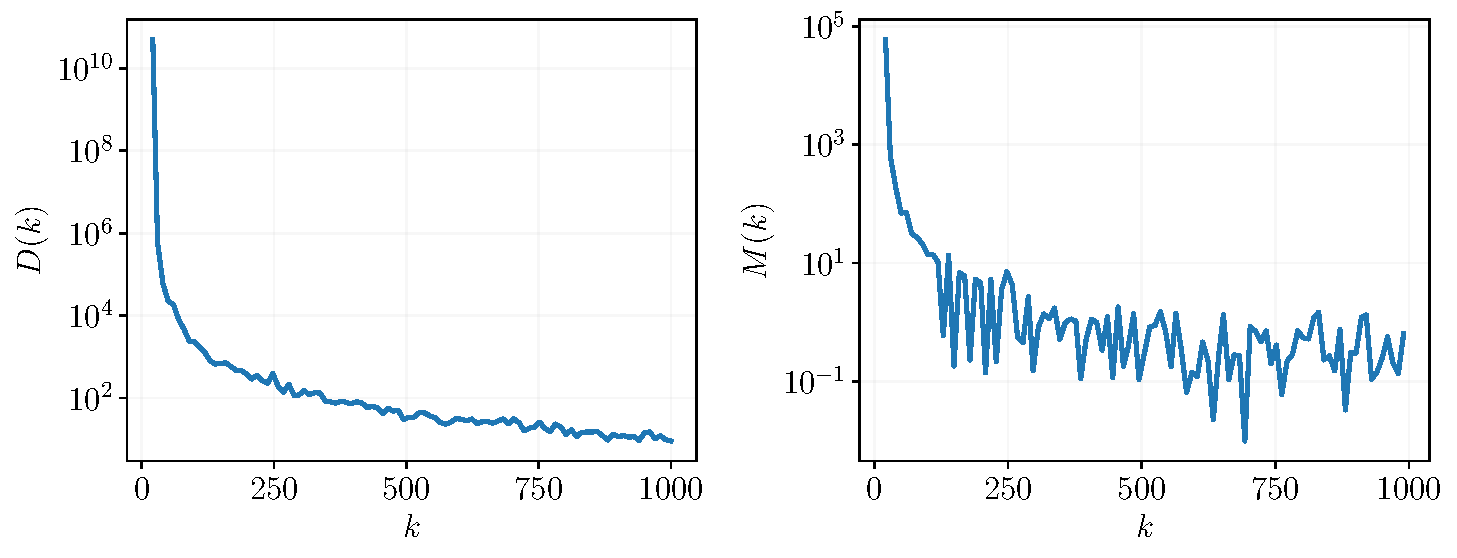
\includegraphics[width=\textwidth]{likelihood-synthetic-regression}
    \caption{Синтетическая выборка (линейная регрессия)}
    \label{likelihood-synthetic-regression}
\end{figure}

\begin{figure}[h!]
    \centering
    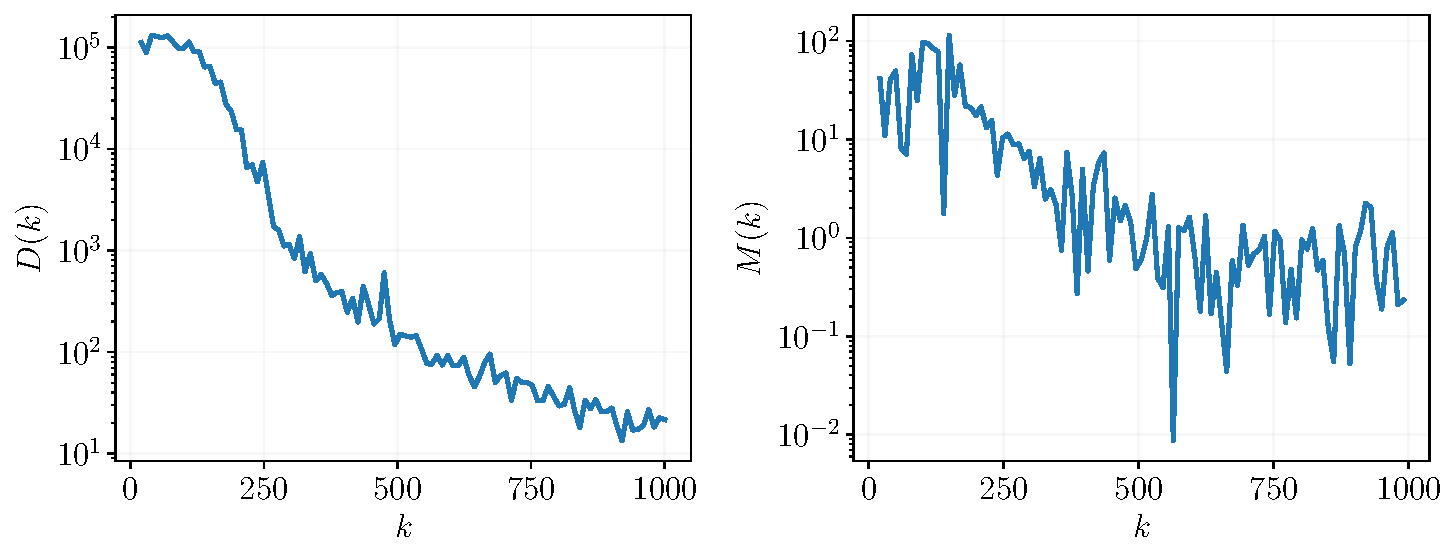
\includegraphics[width=\textwidth]{likelihood-synthetic-classification}
    \caption{Синтетическая выборка (логистическая регрессия)}
    \label{likelihood-synthetic-classification}
\end{figure}

\begin{figure}[h!]
    \centering
    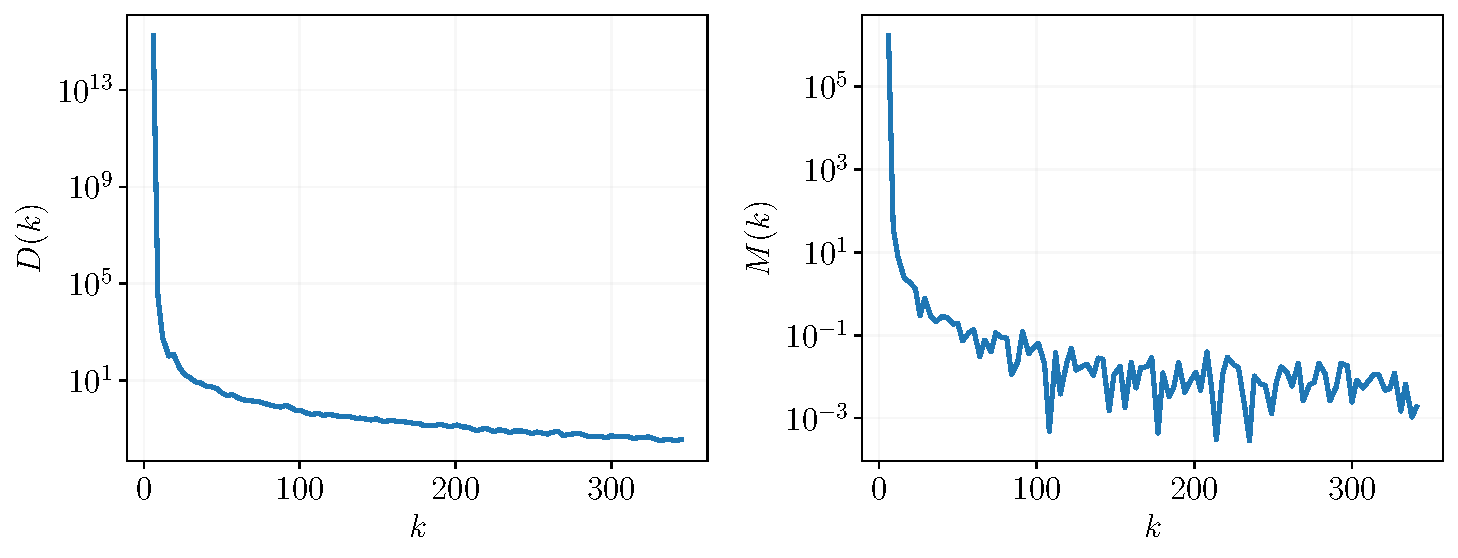
\includegraphics[width=\textwidth]{likelihood-liver-disorders}
    \caption{Выборка Liver Disorders (регрессия)}
    \label{likelihood-liver-disorders}
\end{figure}

\paragraph{Варьирование гиперпараметра $\varepsilon$ для достаточного размера выборки.}

В определениях D-достаточности и M-достаточности участвует гиперпараметр $\varepsilon$, который отвечает за порог для достаточного размера выборки $m^*$. С целью изучения зависимости между ними, мы представляем Рис.~\ref{likelihood-sufficient-vs-threshold}, который демонстрирует, какой размер выборки следует выбрать, чтобы обеспечить определенный уровень уверенности.

\begin{figure}[h!]
    \centering
    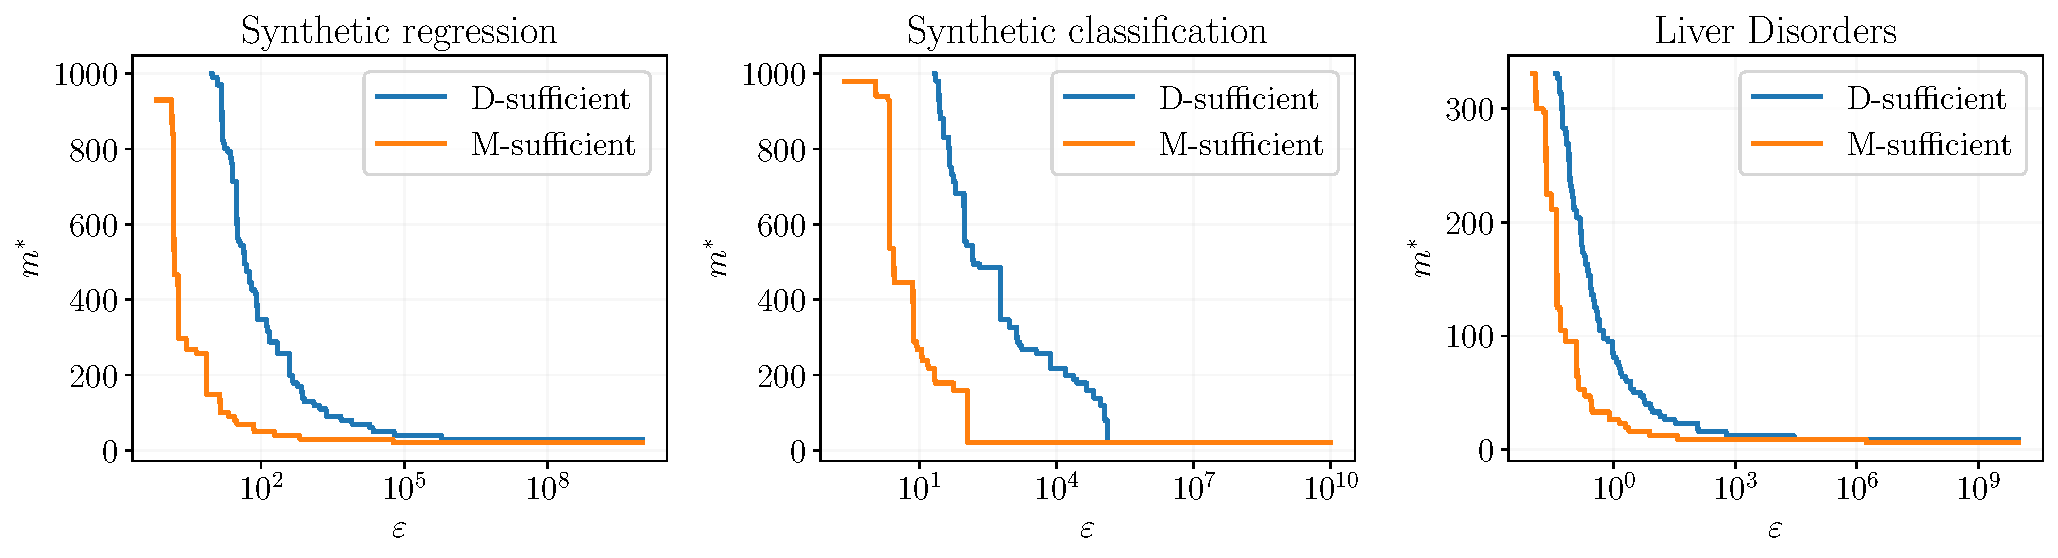
\includegraphics[width=\textwidth]{likelihood-sufficient-vs-threshold}
    \caption{Достаточный размер выборки в зависимости от гиперпараметра $\varepsilon$}
    \label{likelihood-sufficient-vs-threshold}
\end{figure}

\subsubsection{Близость апостериорных распределений}

\paragraph{Сходимость апостериорных распределений.}

Используется синтетическая выборка, сгенерированная из модели линейной регрессии. С целью упрощения визуализации рассматриваются одномерный и двумерный случаи. Число объектов 100, среднеквадратичное отклонение шума 1, априорное распределение параметров $\mathcal{N}(\bw | \mathbf{0}, \bI)$. Далее представлены Рис.~\ref{posterior-1d-similarity} и Рис.~\ref{posterior-2d-similarity}, на которых изображено сходство апостериорных распределений, определенных на схожих подвыборках размера $k$ и $k+1$.

\begin{figure}[h!]
    \centering
    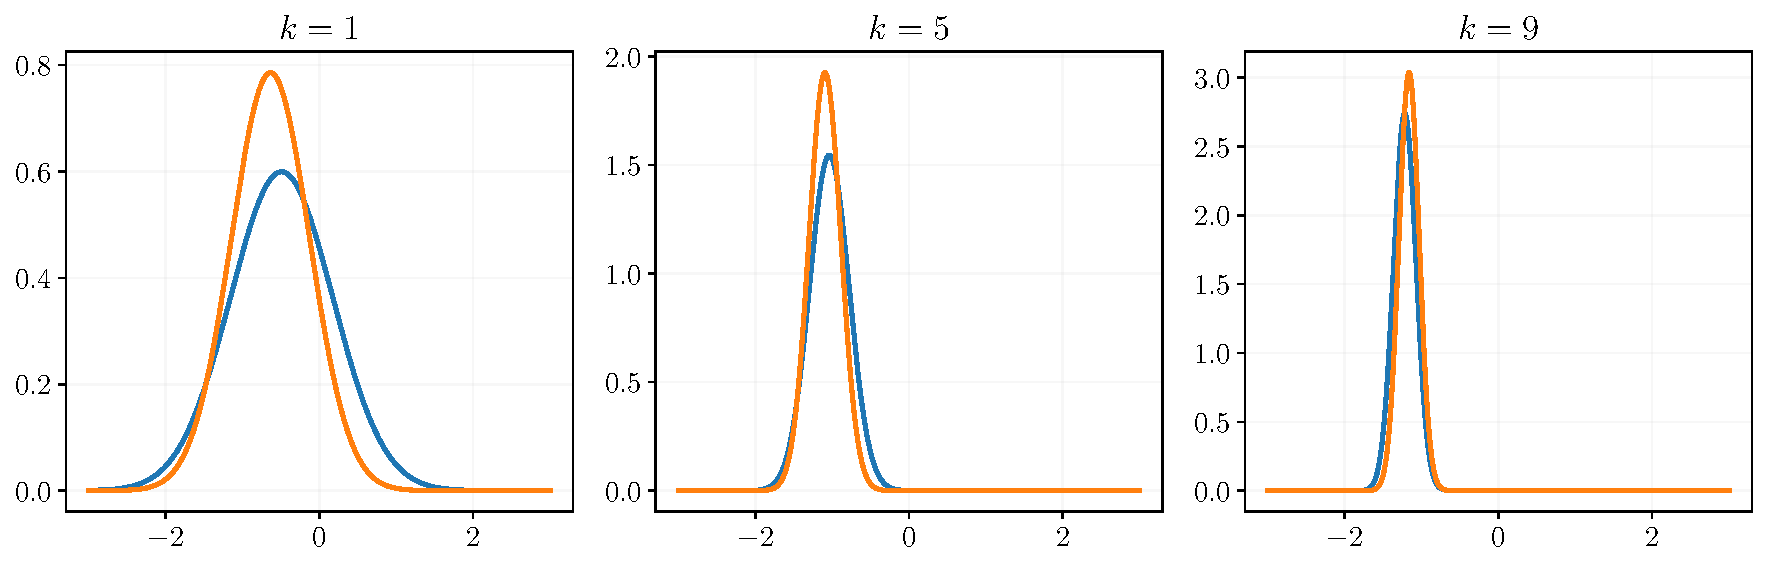
\includegraphics[width=\textwidth]{posterior-1d-similarity}
    \caption{Апостериорные распределения параметров на схожих подвыборках (одномерный случай~--- графики плотностей распределения)}
    \label{posterior-1d-similarity}
\end{figure}

\begin{figure}[h!]
    \centering
    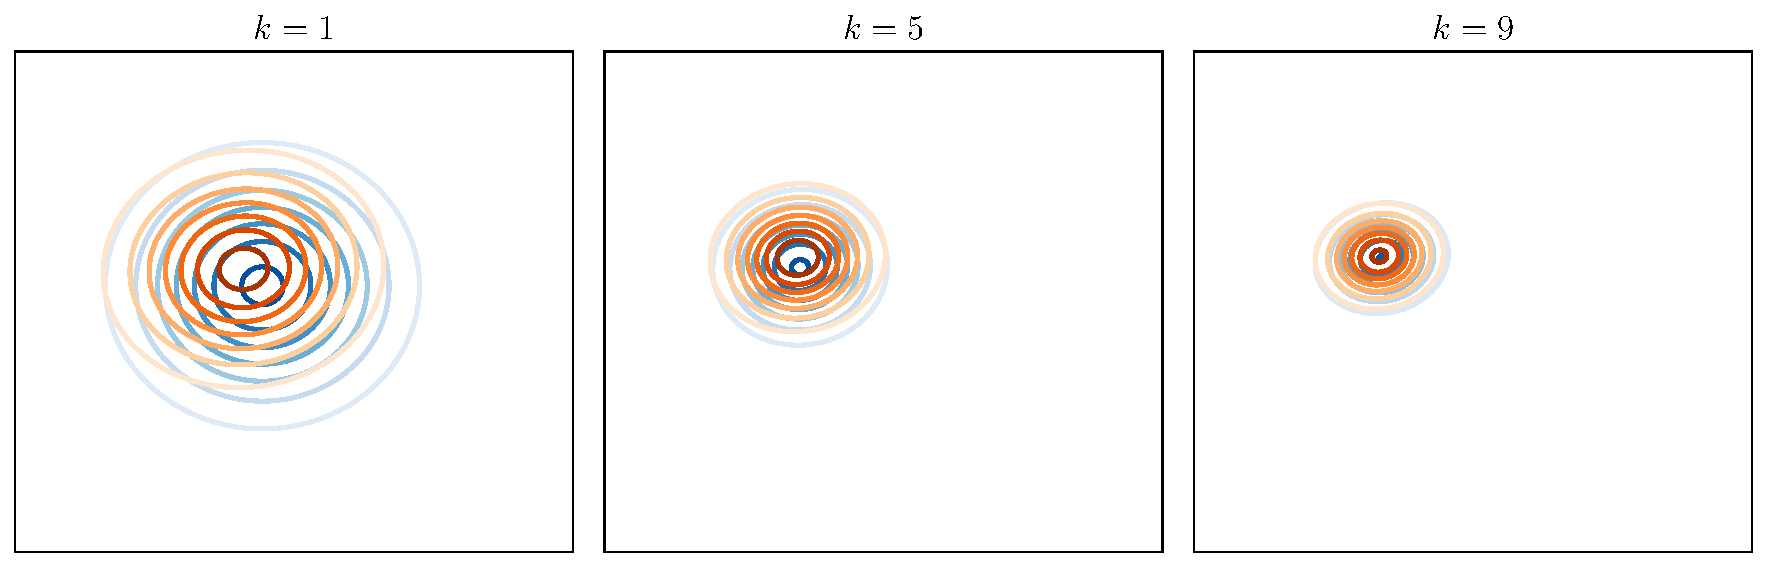
\includegraphics[width=\textwidth]{posterior-2d-similarity}
    \caption{Апостериорные распределения параметров на схожих подвыборках (двумерный случай~--- графики линий уровня)}
    \label{posterior-2d-similarity}
\end{figure}

Видно, что в обоих случаях распределение параметров становится схожим при росте доступного размера выборки. Эта интуиция и послужила фундаментом для предложенных в настоящей работе методов.

\paragraph{Асимптотическое поведение минимального собственного значения матрицы $\bX\T\bX$.}

Синтетические данные сгенерированы из модели линейной регрессии. Число объектов 500, число признаков 10. Один объект последовательно удаляется из данной выборки, пока число объектов в подвыборке не станет равно числу признаков. Для каждого размера выборки $k$ подсчитывается минимальное собственное значение матрицы $\mathbf{X}_k\T \mathbf{X}_k$. Кроме того, подсчитываются значения функций $KL(k)$ и $S(k)$. Такой процесс повторяется $B=100$ раз.

Датасет с задачей регрессии Liver Disorders из \cite{UCI} имеет 345 объектов и 5 признаков. Мы аналогично удаляем объекты из выборки один за другим. Подсчитываются минимальное собственное значение и значения функций. Процесс повторяется $B=1000$ раз.

Рис.~\ref{posterior-eigvals} показывает асимптотическое поведение минимального собственного значения матрицы $\mathbf{X}_k\T \mathbf{X}_k$. Видно, что при стремлении размера выборки к бесконечности минимальное собственное значение также стремится к бесконечности. Помимо этого, как и требуется в Теореме~\ref{theorem4}, этот график лежит выше, чем $\sqrt{k}$.

\begin{figure}[h!]
    \centering
    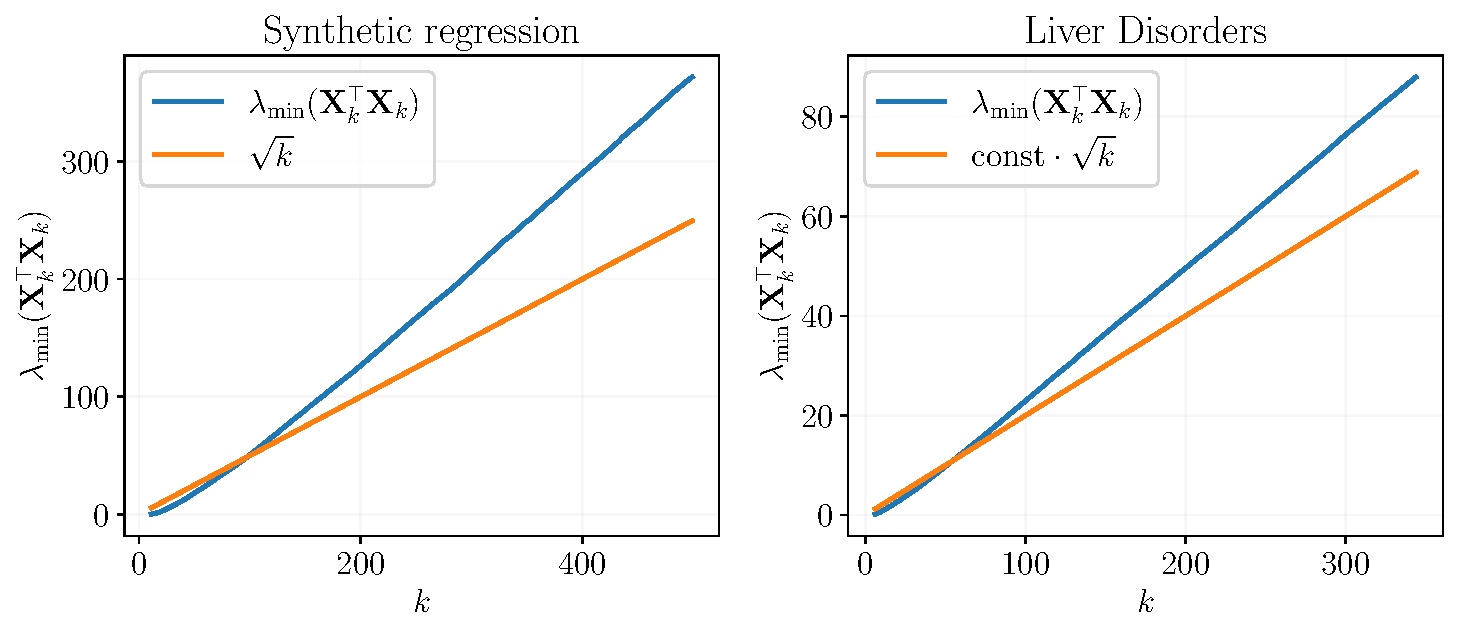
\includegraphics[width=\textwidth]{posterior-eigvals}
    \caption{Минимальное собственное значение матрицы $\mathbf{X}_k\T \mathbf{X}_k$}
    \label{posterior-eigvals}
\end{figure}

\paragraph{Сходимость функций $KL(k)$ и $S(k)$.}

На Рис.~\ref{posterior-synthetic-regression} мы можем наблюдать полученные зависимости между доступным размером выборки $k$ и предложенными функциями $KL(k)$ и $S(k)$ для синтетической выборки с задачей регрессии. В то же время, на Рис.~\ref{posterior-liver-disorders} можно видеть аналогичные графики для датасета Liver Disorders. Для обеих выборок значения функции $KL(k)$ стремятся к нулю при увеличении размера выборки, а значения $S(k)$ стремятся к единице. Эти эмпирические результаты подтверждают теоретические, представленные ранее.

\begin{figure}[h!]
    \centering
    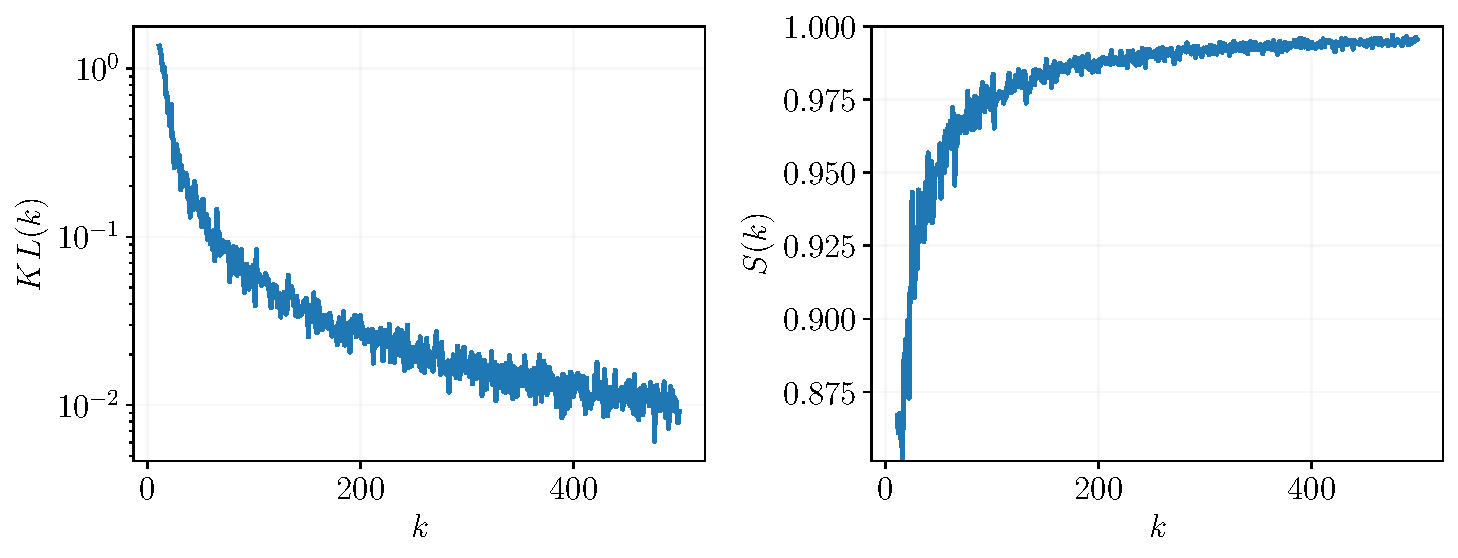
\includegraphics[width=\textwidth]{posterior-synthetic-regression}
    \caption{Синтетическая выборка (линейная регрессия)}
    \label{posterior-synthetic-regression}
\end{figure}

\begin{figure}[h!]
    \centering
    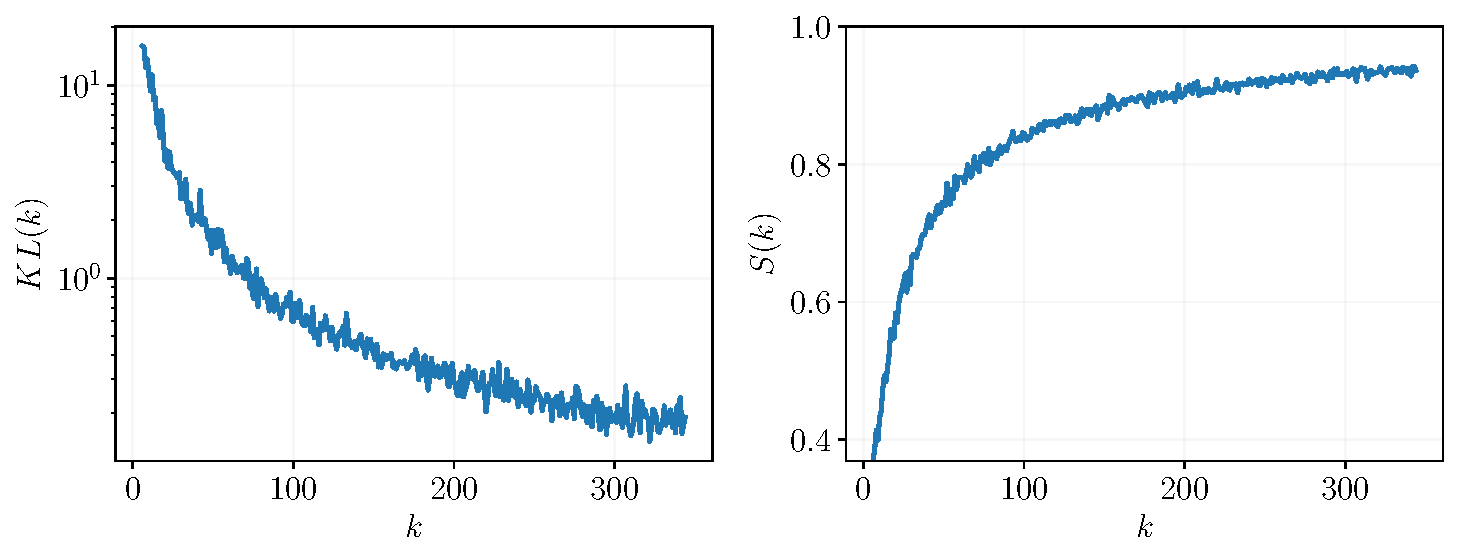
\includegraphics[width=\textwidth]{posterior-liver-disorders}
    \caption{Выборка Liver Disorders (регрессия)}
    \label{posterior-liver-disorders}
\end{figure}

\paragraph{Варьирование гиперпараметра $\varepsilon$ для достаточного размера выборки.}

В определениях KL-достаточности и S-достаточности участвует гиперпараметр $\varepsilon$, который отвечает за порог для достаточного размера выборки $m^*$. С целью изучения зависимости между ними, мы представляем Рис.~\ref{posterior-sufficient-vs-threshold}, который демонстрирует, какой размер выборки следует выбрать, чтобы обеспечить определенный уровень уверенности.

\begin{figure}[h!]
    \centering
    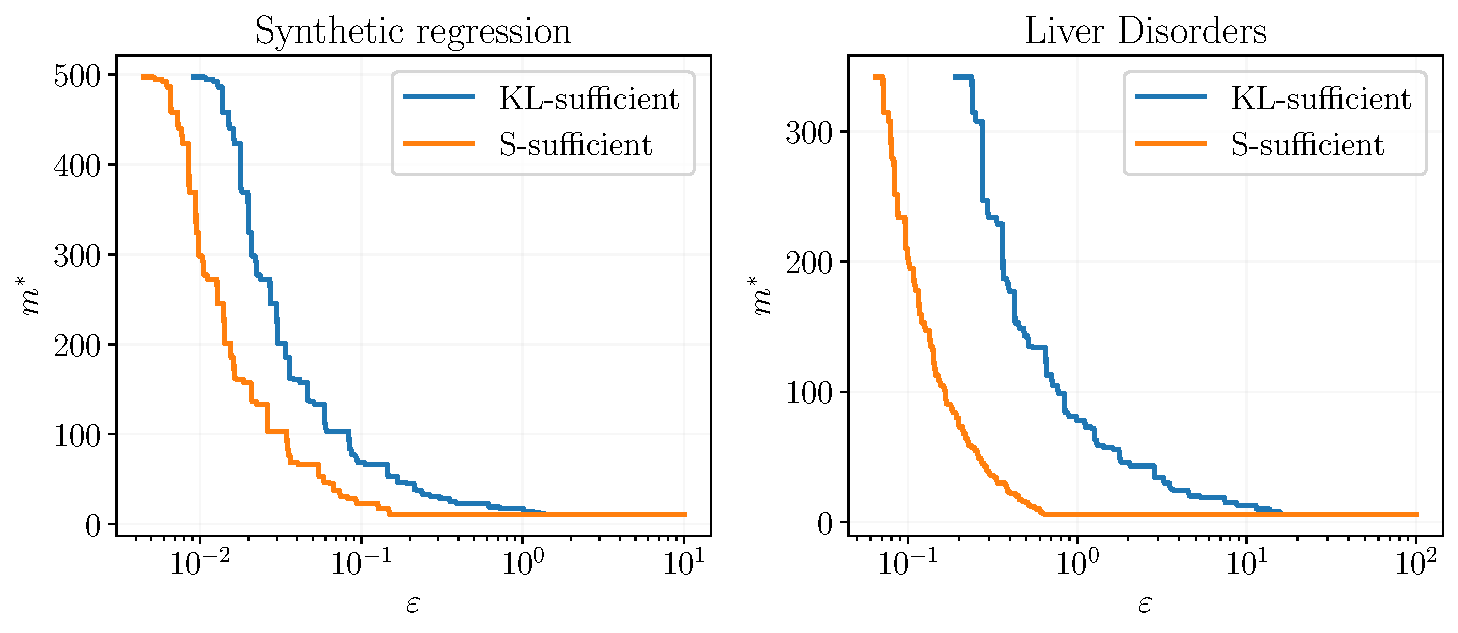
\includegraphics[width=\textwidth]{posterior-sufficient-vs-threshold}
    \caption{Достаточный размер выборки в зависимости от гиперпараметра $\varepsilon$}
    \label{posterior-sufficient-vs-threshold}
\end{figure}

Для $\varepsilon=10$ достаточно взять число объектов, равное числу признаков. Однако для $\varepsilon=10^{-2}$ требуется взять всю выборку.

\paragraph{Сравнение подходов на множестве выборок.}

Чтобы оценить эффективность предложенных методов на разных наборах данных, были выбраны выборки из открытой библиотеки \cite{UCI}. Подробная информация о каждом наборе данных, количество наблюдений и количество признаков представлены в таблице~\ref{table}. Для демонстрационных целей было выбрано значение гиперпараметра $\varepsilon$, при котором значение целевой функции $KL(k)$ или $S(k)$ уменьшается вдвое. Соответствующие результаты приведены в таблице~\ref{table}. Пропуски означают, что первоначальный размер выборки недостаточен.

\begin{table}
    \centering
    \caption{Выборки с задачей регрессии (пропуски означают, что первоначальный размер выборки недостаточен)}\label{table}
    \begin{tabular}{|c|c|c|c|c|}
    \hline
    Название выборки & Объектов $m$ & Признаков $n$ & KL & S \\
    \hline
    Abalone & 4177 & 8 & 3751 & 3751\\
    Auto MPG & 392 & 8 & 55 & --- \\
    Automobile & 159 & 25 & 152 & --- \\
    Liver Disorders & 345 & 6 & 282 & --- \\
    Servo & 167 & 4 & 138 & 160 \\
    Forest fires & 517 & 12 & 487 & --- \\
    Wine Quality & 6497 & 12 & --- & --- \\
    Energy Efficiency & 768 & 9 & --- & --- \\
    Student Performance & 649 & 32 & --- & --- \\
    Facebook Metrics & 495 & 18 & 379 & 475  \\
    Real Estate Valuation & 414 & 7 & --- & --- \\
    Heart Failure Clinical Records & 299 & 12 & 258 & 293 \\
    Bone marrow transplant: children & 142 & 36 & 109 & --- \\
    \hline
    \end{tabular}
\end{table}

%%% ЭТА ЧАСТЬ НАХОДИТСЯ В РАЗРАБОТКЕ
%%% ПОКА ЧТО ОЧЕНЬ СЫРОЙ МАТЕРИАЛ
\clearpage
\subsection{Достаточный размер выборки больше доступного}

\subsubsection{Определение параметрического семейства функций с помощью генетического алгоритма}

Реализацию генетического алгоритма, приведенного в разделе \ref{ga}, можно найти в \href{https://github.com/kisnikser/Bayesian-Sample-Size-Estimation/tree/main/code/genetic_algorithm}{репозитории}. Для исследования зависимости функции ошибки от используемого размера выборки в задаче регрессии использовались следующие датасеты из \citep{UCI}: Abalone, Auto MPG, Liver Disorders, Wine Quality, Parkinsons Telemonitoring, Bike Sharing Dataset, Real estate valuation и Heart failure clinical records. Была выбрана квадратичная функция потерь MSE. Задача регрессии для каждого из них решалась с помощью линейной регрессии из \citep{scikit-learn}. Усреднение производилось по $B = 100$ бутстрап-выборкам. Как было сказано ранее, все зависимости приводятся к одинаковому масштабу по обеим осям. Полученные графики представлены на Рис.~\ref{datasets-regression}. Слева находится график для выборочного среднего. Справа находится график для выборочного среднеквадратичного отклонения.

\begin{figure}[h!]
    \centering
    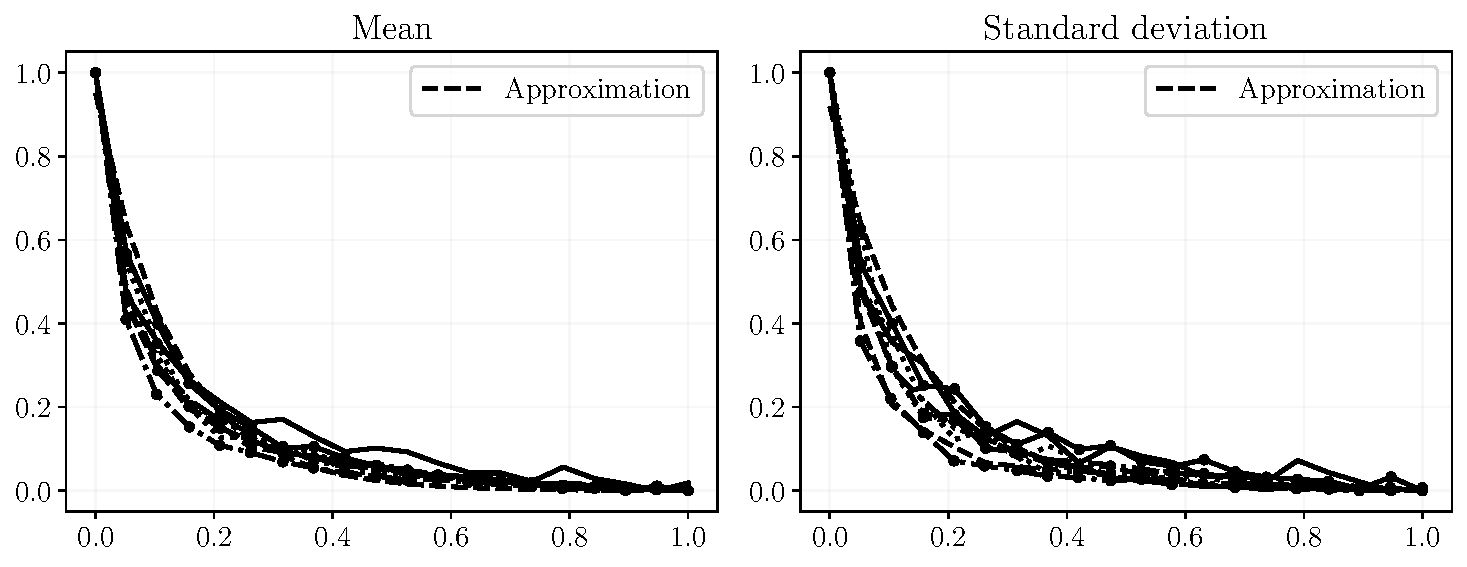
\includegraphics[width=\textwidth]{datasets-regression}
    \caption{Поведение функции ошибки в задаче регрессии}
    \label{datasets-regression}
\end{figure}

Применение генетического алгоритма приводит к одинаковому семейству функций для аппроксимации среднего и среднеквадратичного отклонения в задаче регрессии:
\[ w_0 + w_1 \cdot \exp(w_2 \cdot x). \]

В задаче классификации использовалось 12 датасетов из \citep{UCI}: Automobile, Breast Cancer Wisconsin (Diagnostic), Car Evaluation, Credit Approval, Glass Identification, Ionosphere, Iris, Tic-Tac-Toe Endgame, Congressional Voting Records, Wine, Zoo и Heart failure clinical records. Задача классификации для каждого из них решалась с помощью логистической регрессии из \citep{scikit-learn}. Усреднение производилось по $B = 100$ бутстрап-выборкам. Все завимисости также приводятся к одинаковому масштабу по обеим осям. Полученные графики представлены на Рис.~\ref{datasets-classification}. Как и ранее, слева находится график для выборочного среднего, справа находится график для выборочного среднеквадратичного отклонения.

\begin{figure}[h!]
    \centering
    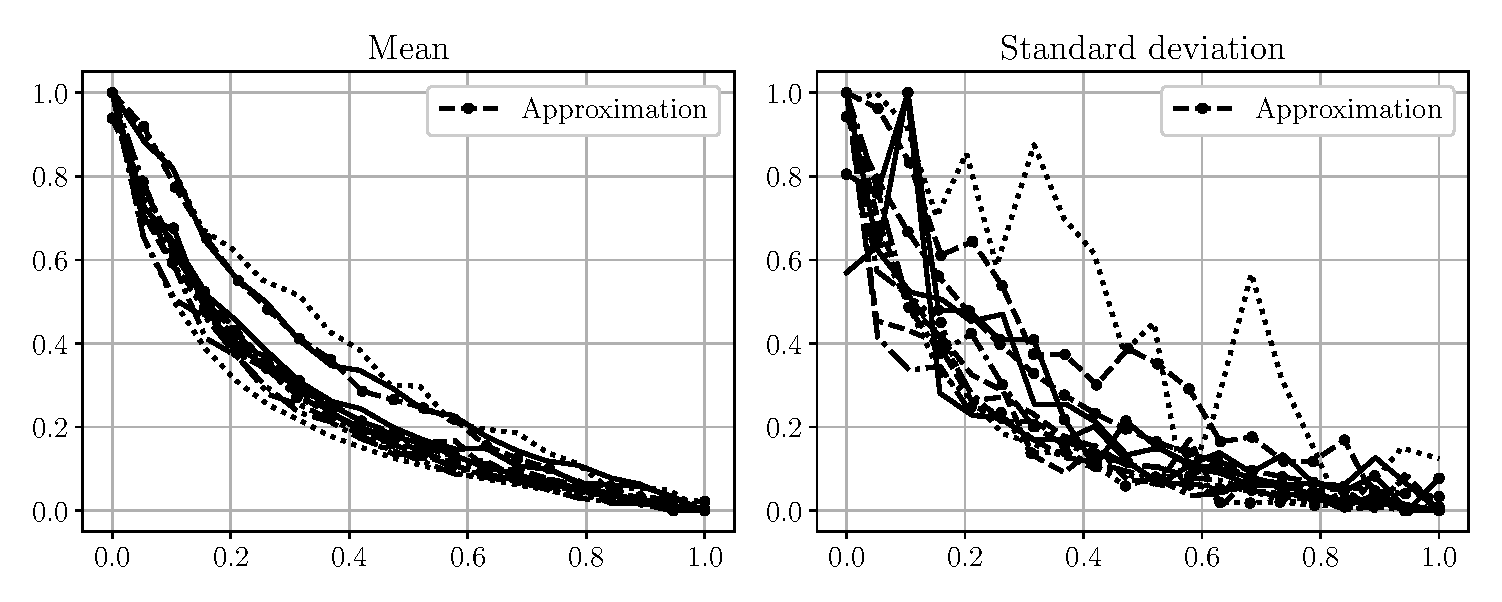
\includegraphics[width=\textwidth]{datasets-classification}
    \caption{Поведение функции ошибки в задаче классификации}
    \label{datasets-classification}
\end{figure}

Применение генетического алгоритма для среднего значения приводит к такому же семейству функций, как и в задаче регрессии:
\[ w_0 + w_1 \cdot \exp(w_2 \cdot x). \]

Среднеквадратичное отклонение в случае задачи классификации для каждой выборки имеет свою зависимость от размера выборки. Таким образом, прогнозировать дисперсию для классификации оказывается достаточно сложной задачей.



%%% Заключение
\section{Заключение}

Предложены подходы к определению достаточного размера выборки, основанные на значениях функции правдоподобия на бустрапированных подвыборках и близости апостериорных распределений параметров модели на схожих подвыборках. Первые два позволяют определять достаточный размер выборки на любом датасете с задачей регрессии или классификации. Доказана корректность предложенных подходов при определенных ограничениях на используемую модель, а также предложен метод прогнозирования функции правдоподобия в случае недостаточного размера выборки. Доказана теорема о моментах предельного апостериорного распределения параметров в модели линейной регрессии. Проведенный вычислительный эксперимент позволяет анализировать свойства предложенных методов и их эффективность. Определено параметрическое семейство функций, аппроксимирующее функцию ошибки для набора датасетов. 

%%% Список литературы
\bibliographystyle{unsrtnat}
\bibliography{references}

%%% Приложение
\newpage
\cleardoublepage
\phantomsection
\addcontentsline{toc}{section}{Приложение}    % Добавляем его в оглавление
\section*{Приложение}\label{append}                       % Заголовок

\begin{proof}[Доказательство (Теорема \ref{theorem1})]
    Рассмотрим определение M-достаточного размера выборки в терминах логарифма функции правдоподобия. В модели линейной регрессии
    \[ L\left( \mathfrak{D}_m, \hat{\bw}_k \right) = p(\by | \bX, \hat{\bw}_k) = \prod_{i=1}^{m} p(y_i | \bx_i, \hat{\bw}_k) = \prod_{i=1}^{m} \mathcal{N}\left( y_i | \hat{\bw}_k\T \bx_i, \sigma^2 \right) = \]
    \[ = \left( 2\pi\sigma^2 \right)^{-m/2} \exp\left( -\dfrac{1}{2\sigma^2} \| \by - \bX \hat{\bw}_k \|_2^2 \right). \]
    Прологарифмируем:
    \[ l\left( \mathfrak{D}_m, \hat{\bw}_k \right) = \log p(\by | \bX, \hat{\bw}_k) = -\dfrac{m}{2}\log\left( 2\pi\sigma^2 \right) - \dfrac{1}{2\sigma^2} \| \by - \bX \hat{\bw}_k \|_2^2. \]
    Возьмем математическое ожидание по $\mathfrak{D}_k$, учитывая, что $\mathbb{E} \hat{\bw}_k = \bm_k$ и $\mathbb{D} \hat{\bw}_k = \bSigma_k$:
    \[ \mathbb{E}_{\hat{\mathbf{w}}_{k}} l\left( \mathfrak{D}_m, \hat{\bw}_k \right) = -\dfrac{m}{2}\log\left( 2\pi\sigma^2 \right) - \dfrac{1}{2\sigma^2} \Big( \| \by - \bX \bm_k \|_2^2 + \text{tr}\left( \bX\T\bX \bSigma_k \right) \Big). \]
    Запишем выражение для разности математических ожиданий:
    \[ \mathbb{E}_{\hat{\mathbf{w}}_{k+1}} l(\mathfrak{D}_m, \hat{\mathbf{w}}_{k+1}) - \mathbb{E}_{\hat{\mathbf{w}}_{k}} l(\mathfrak{D}_m, \hat{\mathbf{w}}_{k}) = \]
    \[ = \dfrac{1}{2\sigma^2} \Big( \| \by - \bX \bm_k \|_2^2 - \| \by - \bX \bm_{k+1} \|_2^2 \Big) + \dfrac{1}{2\sigma^2} \text{tr} \Big( \bX\T\bX \left( \bSigma_k - \bSigma_{k+1} \Big) \right) = \]
    \[ = \dfrac{1}{2\sigma^2} \Big( 2 \by\T \bX (\bm_{k+1} - \bm_k) + (\bm_k - \bm_{k+1})\T \bX\T\bX (\bm_k + \bm_{k+1}) \Big) + \]
    \[ + \dfrac{1}{2\sigma^2} \text{tr} \Big( \bX\T\bX \left( \bSigma_k - \bSigma_{k+1} \right) \Big). \]
    Значение функции $M(k)$ есть модуль от вышеприведенного выражения. Применим неравенство треугольника для модуля, а затем оценим каждое слагаемое.\\
    Первое слагаемое оценим, используя неравенство Коши-Буняковского:
    \[ \big| \by\T\bX(\bm_{k+1}-\bm_k) \big| \leqslant \| \bX\T\by \|_2 \|\bm_{k+1} - \bm_k\|_2. \]
    Второе слагаемое оценим, используя неравенство Коши-Буняковского, свойство согласованности спектральной матричной нормы, а также ограниченность последовательности векторов $\bm_k$, которая следует из предъявленной в условии сходимости:
    \[ \big| (\bm_k - \bm_{k+1})\T \bX\T\bX (\bm_k + \bm_{k+1}) \big| \leqslant \| \bX (\bm_k - \bm_{k+1}) \|_2 \| \bX (\bm_k + \bm_{k+1}) \|_2 \leqslant \]
    \[ \leqslant \| \bX \|_2^2 \| \bm_k - \bm_{k+1} \|_2 \| \bm_k + \bm_{k+1} \|_2 \leqslant C \| \bX \|_2^2 \| \bm_k - \bm_{k+1} \|_2. \]
    Последнее слагаемое оценим, используя неравенство Гельдера для нормы Фробениуса:
    \[ \Big| \text{tr} \Big( \bX\T\bX \left( \bSigma_k - \bSigma_{k+1} \right) \Big) \Big| \leqslant \| \bX\T\bX \|_F \| \bSigma_k - \bSigma_{k+1} \|_F. \]
    Наконец, поскольку $\| \bm_k - \bm_{k+1} \|_2 \to 0$ и $\| \bSigma_k - \bSigma_{k+1} \|_{F} \to 0$ при $k \to \infty$, то $M(k) \to 0$ при $k \to \infty$, что доказывает теорему.
\end{proof}

\begin{proof}[Доказательство (Следствие)]
    Из приведенных в условии сходимостей следует, что $\| \bm_k - \bm_{k+1} \|_2 \to 0$ и $\| \bSigma_k - \bSigma_{k+1} \|_{F} \to 0$ при $k \to \infty$. Применение Теоремы \ref{theorem1} заканчивает доказательство.
\end{proof}

\begin{proof}[Доказательство (Теорема \ref{theorem2})]
    Дивергенция Кульбака-Лейблера для пары нормальных апостериорных распределений имеет вид
    \[ D_{\text{KL}}\left( p_k \| p_{k+1} \right) = \dfrac{1}{2} \Big( \mathrm{tr}\left( \mathbf{\Sigma}_{k+1}^{-1} \mathbf{\Sigma}_k \right) + (\mathbf{m}_{k+1} - \mathbf{m}_k)\T \mathbf{\Sigma}_{k+1}^{-1} (\mathbf{m}_{k+1} - \mathbf{m}_k) - \]
    \[ - n + \log{\left( \dfrac{\det \mathbf{\Sigma}_{k+1}}{\det \mathbf{\Sigma}_{k}} \right)} \Big). \]
    Представим $\bSigma_{k+1}$ как $\bSigma_{k+1} = \bSigma_k + \Delta \bSigma$. Рассмотрим в отдельности каждое слагаемое.
    \[ \mathrm{tr}\left( \mathbf{\Sigma}_{k+1}^{-1} \mathbf{\Sigma}_k \right) = \mathrm{tr}\left( \left( \mathbf{\Sigma}_k + \Delta \bSigma \right)^{-1} \mathbf{\Sigma}_k \right) \to \mathrm{tr} \mathbf{I}_n= n \text{ при } \| \Delta \bSigma \|_F \to 0, \]
    \[ \left| (\mathbf{m}_{k+1} - \mathbf{m}_k)\T \mathbf{\Sigma}_{k+1}^{-1} (\mathbf{m}_{k+1} - \mathbf{m}_k) \right| \leqslant \| \mathbf{m}_{k+1} - \mathbf{m}_k \|_2^2 \| \mathbf{\Sigma}_{k+1}^{-1} \|_2 \to 0 \] 
    при $ \mathbf{m}_{k+1} - \mathbf{m}_k \|_2 \to 0$,
    \[ \log{\left( \dfrac{\det \mathbf{\Sigma}_{k+1}}{\det \mathbf{\Sigma}_{k}} \right)} = \log{\left( \dfrac{\det \left( \mathbf{\Sigma}_k + \Delta \bSigma \right)}{\det \mathbf{\Sigma}_{k}} \right)} \to \log \det \mathbf{I}_n = \log 1 = 0 \]
    при $ \Delta \bSigma \|_F \to 0$, откуда и имеем требуемое.
\end{proof}

\begin{proof}[Доказательство (Теорема \ref{theorem3})]
    Воспользуемся выражением s-score для пары нормальных априорных распределений из \cite{Aduenko2017}:
    \[ \text{s-score}(p_k, p_{k+1}) = \exp{\left( -\dfrac{1}{2} (\mathbf{m}_{k+1} - \mathbf{m}_k)\T \left( \mathbf{\Sigma}_k + \mathbf{\Sigma}_{k+1} \right)^{-1} (\mathbf{m}_{k+1} - \mathbf{m}_k) \right)}. \]
    Поскольку
    \[ \left| (\mathbf{m}_{k+1} - \mathbf{m}_k)\T \left( \mathbf{\Sigma}_k + \mathbf{\Sigma}_{k+1} \right)^{-1} (\mathbf{m}_{k+1} - \mathbf{m}_k) \right| \leqslant \]
    \[ \leqslant \| \mathbf{m}_{k+1} - \mathbf{m}_k \|_2^2 \| \left( \mathbf{\Sigma}_k + \mathbf{\Sigma}_{k+1} \right)^{-1} \|_2 \to 0 \]
    при $\| \mathbf{m}_{k+1} - \mathbf{m}_k \|_2 \to 0$, то значение квадратичной формы внутри экспоненты стремится к нулю. Следовательно, $\text{s-score}(p_k, p_{k+1}) \to 1$ при устремлении $\| \mathbf{m}_{k+1} - \mathbf{m}_k \|_2 \to 0$.
\end{proof}

\begin{proof}[Доказательство (Теорема \ref{theorem4})]
    Пусть задано нормальное априорное распределение параметров $p(\bw) = \mathcal{N}\left( \bw | \mathbf{0}, \alpha^{-1} \bI \right)$. В модели линейной регрессии правдоподобие является нормальным, а именно
    \[ p(\by | \bX, \bw) = \mathcal{N}\left( \by | \bX \bw, \sigma^2 \mathbf{I} \right) = \left( 2\pi\sigma^2 \right)^{-m/2} \exp\left( -\dfrac{1}{2\sigma^2} \| \by - \bX \bw \|_2^2 \right). \]
    Используя сопряженность априорного распределения и правдоподобия, легко найти параметры апостериорного распределения:
    \[ p(\bw | \bX, \by) = \mathcal{N}\left( \bw | \bm, \bSigma \right), \]
    где
    \[ \bSigma = \left( \alpha \bI + \dfrac{1}{\sigma^2} \bX\T \bX \right)^{-1}, \qquad \bm = \left( \bX\T \bX + \alpha \sigma^2 \bI \right)^{-1} \bX\T \by. \]
    Рассмотрим выражение $\| \bSigma_{k+1} - \bSigma_k \|_2$ нормы разности матриц ковариции для подвыборок размера $k$ и $k+1$. Введем обозначение $\bA_k = \dfrac{1}{\sigma^2} \bX\T_k \bX_k$. Учитывая формулы выше, имеем
    \[ \| \bSigma_{k+1} - \bSigma_k \|_2 = \left\| \left( \alpha \bI + \bA_{k+1} \right)^{-1} - \left( \alpha \bI + \bA_k \right)^{-1} \right\|_2 = \]
    \[ = \left\| \left( \alpha \bI + \bA_{k+1} \right)^{-1} \left( \bA_{k+1} - \bA_k \right) \left( \alpha \bI + \bA_k \right)^{-1} \right\|_2 \leqslant \]
    Воспользуемся субмультипликативностью спектральной матричной нормы.
    \[ \leqslant \left\| \left( \alpha \bI + \bA_{k+1} \right)^{-1} \right\|_2 \left\| \left( \alpha \bI + \bA_k \right)^{-1} \right\|_2 \left\| \bA_{k+1} - \bA_k \right\|_2 = \]
    Теперь воспользуемся выражением спектральной матричной нормы через максимальное собственное значение.
    \[ = \dfrac{1}{\lambda_{\min}\left( \alpha \bI + \bA_{k+1} \right)} \dfrac{1}{\lambda_{\min}\left( \alpha \bI + \bA_k \right)} \left\| \bA_{k+1} - \bA_k \right\|_2 \leqslant \]
    \[ \leqslant \dfrac{1}{\lambda_{\min}\left( \bA_{k+1} \right)} \dfrac{1}{\lambda_{\min}\left( \bA_k \right)} \left\| \bA_{k+1} - \bA_k \right\|_2 = \]
    \[ = \sigma^2  \dfrac{1}{\lambda_{\min}\left( \bX\T_{k+1} \bX_{k+1} \right)} \dfrac{1}{\lambda_{\min}\left( \bX\T_k \bX_k \right)} \left\| \bX\T_{k+1} \bX_{k+1} - \bX\T_k \bX_k \right\|_2. \]
    Далее, поскольку по условию $\| \bx \|_2 \leqslant M$, то
    \[ \left\| \bX\T_{k+1} \bX_{k+1} - \bX\T_k \bX_k \right\|_2 = \left\| \sum\limits_{i=1}^{k+1} \bx_i \bx_i\T - \sum\limits_{i=1}^{k} \bx_i \bx_i\T \right\|_2 = \left\| \bx_{k+1} \bx_{k+1}\T \right\|_2 = \]
    Матрица единичного ранга имеет единственное ненулевое собственное значение.
    \[ = \lambda_{\max}\left( \bx_{k+1} \bx_{k+1}\T \right)  = \bx_{k+1}\T \bx_{k+1} = \| \bx_{k+1} \|_2^2 \leqslant M^2. \]
    По условию $\lambda_{\min}\left( \bX\T_k \bX_k \right) = \omega(\sqrt{k})$, тогда $\| \bSigma_{k+1} - \bSigma_k \|_2 = o(k^{-1})$ при $k \to \infty$. Далее воспользуемся эквивалентностью матричных норм, а именно
    \[ \| \bSigma_{k+1} - \bSigma_k \|_F \leqslant \sqrt{k} \| \bSigma_{k+1} - \bSigma_k \|_2 = o(k^{-1/2}) \text{ при } k \to \infty, \]
    что и требовалось доказать. Теперь оценим норму разности математических ожиданий.
    \[ \| \bm_{k+1} - \bm_k \|_2 = \left\| \left( \bX_{k+1}\T \bX_{k+1} + \alpha \sigma^2 \bI \right)^{-1} \bX_{k+1}\T \by_{k+1} - \left( \bX_k\T \bX_k + \alpha \sigma^2 \bI \right)^{-1} \bX_k\T \by_k \right\|_2 = \]
    Учтем, что $\bX_{k+1}\T = [\bX_k\T, \bx_{k+1}]$ и $\by_{k+1} = [\by_k, y_{k+1}]\T$, тогда $\bX_{k+1}\T \bX_{k+1} = \bX_k\T \bX_k + \bx_{k+1} \bx_{k+1}\T$ и $\bX_{k+1}\T \by_{k+1} = \bX_k\T \by_k + \bx_{k+1} y_{k+1}$.
    \[ = \left\| \left( \bX_k\T \bX_k + \alpha \sigma^2 \bI + \bx_{k+1} \bx_{k+1}\T \right)^{-1} \left( \bX_k\T \by_k + \bx_{k+1} y_{k+1} \right) - \left( \bX_k\T \bX_k + \alpha \sigma^2 \bI \right)^{-1} \bX_k\T \by_k \right\|_2 = \]
    Вынесем множитель в первом слагаемом:
    \[ \left( \bX_k\T \bX_k + \alpha \sigma^2 \bI + \bx_{k+1} \bx_{k+1}\T \right)^{-1} = \left( \bI + \left( \bX_k\T \bX_k + \alpha \sigma^2 \bI \right)^{-1} \bx_{k+1} \bx_{k+1}\T \right)^{-1} \cdot \] 
    \[ \cdot \left( \bX_k\T \bX_k + \alpha \sigma^2 \bI \right)^{-1}.\]
    Далее вынесем общий множитель у обоих слагаемых.
    \begin{multline*}
        = \Bigg\| \left[ \left( \bI + \left( \bX_k\T \bX_k + \alpha \sigma^2 \bI \right)^{-1} \bx_{k+1} \bx_{k+1}\T \right)^{-1} - \bI \right] \left( \bX_k\T \bX_k + \alpha \sigma^2 \bI \right)^{-1} \bX_k\T \by_k + \\ + \left( \bX_{k+1}\T \bX_{k+1} + \alpha \sigma^2 \bI \right)^{-1} \bx_{k+1} y_{k+1} \Bigg\|_2 =
    \end{multline*}
    Воспользуемся неравенством треугольника, а также свойством согласованности и субмультипликативности спектральной нормы.
    \begin{multline*}
        \leqslant \left\| \left( \bI + \left( \bX_k\T \bX_k + \alpha \sigma^2 \bI \right)^{-1} \bx_{k+1} \bx_{k+1}\T \right)^{-1} - \bI \right\|_2 \left\| \left( \bX_k\T \bX_k + \alpha \sigma^2 \bI \right)^{-1} \right\|_2 \left\| \bX_k\T \by_k \right\|_2 + \\ + \left\| \left( \bX_{k+1}\T \bX_{k+1} + \alpha \sigma^2 \bI \right)^{-1} \right\|_2 \left\| \bx_{k+1} y_{k+1} \right\|_2
    \end{multline*}
    Оценим по отдельности каждое слагаемое. В первом множителе первого слагаемого применим формулу для разности обратных матриц, как мы делали с ковариационными матрицами.
    \[ \left\| \left( \bI + \left( \bX_k\T \bX_k + \alpha \sigma^2 \bI \right)^{-1} \bx_{k+1} \bx_{k+1}\T \right)^{-1} - \bI \right\|_2 \leqslant \]
    \[ \leqslant \left\| \left( \bI + \left( \bX_k\T \bX_k + \alpha \sigma^2 \bI \right)^{-1} \bx_{k+1} \bx_{k+1}\T \right)^{-1} \right\|_2 \cdot \left\| \bI \right\|_2 \cdot \left\| \left( \bX_k\T \bX_k + \alpha \sigma^2 \bI \right)^{-1} \bx_{k+1} \bx_{k+1}\T \right\|_2 \leqslant \]
    Снова используем субмультипликативность, а также выражение для нормы матрицы единичного ранга.
    \[ \leqslant \dfrac{1}{\lambda_{\min}\left( \bI + \left( \bX_k\T \bX_k + \alpha \sigma^2 \bI \right)^{-1} \bx_{k+1} \bx_{k+1}\T \right)} \dfrac{\left\| \bx_{k+1} \right\|_2^2}{\lambda_{\min}\left( \bX_k\T \bX_k + \alpha \sigma^2 \bI \right)} \leqslant \]
    \[ \leqslant \dfrac{1}{1 + \lambda_{\min}\left(\left( \bX_k\T \bX_k + \alpha \sigma^2 \bI \right)^{-1} \bx_{k+1} \bx_{k+1}\T \right)} \dfrac{M^2}{\lambda_{\min}\left( \bX_k\T \bX_k \right)} \leqslant \]
    Минимальное собственное значение произведения матриц оценивается произведением их минимальных собственных значений. Кроме того, минимальное собственное значение матрицы единичного ранга $\bx_{k+1} \bx_{k+1}\T$ равно нулю.
    \[ \leqslant \dfrac{1}{1 + \lambda_{\max}\left( \bX_k\T \bX_k + \alpha \sigma^2 \bI \right) \lambda_{\min}\left( \bx_{k+1} \bx_{k+1}\T \right)} \dfrac{M^2}{\lambda_{\min}\left( \bX_k\T \bX_k \right)} = \dfrac{M^2}{\lambda_{\min}\left( \bX_k\T \bX_k \right)}. \]
    Второй и третий множители первого слагаемого оцениваются следующим образом.
    \[ \left\| \left( \bX_k\T \bX_k + \alpha \sigma^2 \bI \right)^{-1} \right\|_2 \left\| \bX_k\T \by_k \right\|_2 \leqslant \dfrac{\left\| \bX_k\T \by_k \right\|_2}{\lambda_{\min}\left( \bX_k\T \bX_k \right)} = \dfrac{\left\| \sum\limits_{i=1}^{k} \bx_i y_i \right\|_2}{\lambda_{\min}\left( \bX_k\T \bX_k \right)} \leqslant \dfrac{k M^2}{\lambda_{\min}\left( \bX_k\T \bX_k \right)} \]
    Наконец, оценим второе слагаемое.
    \[ \left\| \left( \bX_{k+1}\T \bX_{k+1} + \alpha \sigma^2 \bI \right)^{-1} \right\|_2 \left\| \bx_{k+1} y_{k+1} \right\|_2 \leqslant \dfrac{M^2}{\lambda_{\min}\left( \bX_{k+1}\T \bX_{k+1} \right)} \]
    Итого, имеем следующую оценку.
    \[ \| \bm_{k+1} - \bm_k \|_2 \leqslant \dfrac{k M^3}{\lambda_{\min}^2\left( \bX_k\T \bX_k \right)} + \dfrac{M^2}{\lambda_{\min}\left( \bX_{k+1}\T \bX_{k+1} \right)} = k \cdot o(k^{-1}) + o(k^{-1/2}) = o(1) \]
    при $k \to \infty$. Таким образом, получили требуемую сходимость.
\end{proof}

\begin{proof}[Доказательство (Теорема \ref{theorem5})]
    Задано нормальное априорное распределение параметров $p(\bw) = \mathcal{N}\left( \bw | \mathbf{0}, \alpha^{-1} \bI \right)$. Для модели линейной регрессии 
    \[ p(\by | \bX, \bw) = \mathcal{N}\left( \by | \bX \bw, \sigma^2 \mathbf{I} \right) = \left( 2\pi\sigma^2 \right)^{-m/2} \exp\left( -\dfrac{1}{2\sigma^2} \| \by - \bX \bw \|_2^2 \right). \]
    Апостериорное распределение параметров:
    \[ p(\bw | \bX, \by) = \mathcal{N}\left( \bw | \bm, \bSigma \right), \]
    где
    \[ \bSigma = \left( \alpha \bI + \dfrac{1}{\sigma^2} \bX\T \bX \right)^{-1}, \qquad \bm = \left( \bX\T \bX + \alpha \sigma^2 \bI \right)^{-1} \bX\T \by. \]
    Полный байесовский прогноз для одиночной модели выражается по формуле
    \[ p(\mathbf{y}_{\text{test}}|\mathbf{X_{\text{test}}}, \mathbf{X}_k, \mathbf{y}_k) = \int p(\mathbf{y}_{\text{test}}|\mathbf{X_{\text{test}}}, \mathbf{w}) p(\mathbf{w}|\mathbf{X}_k, \mathbf{y}_k) d\mathbf{w} = \]
    \[ = \int \mathcal{N}\left( \mathbf{y}_{\text{test}} | \mathbf{X}_{\text{test}}\mathbf{w}, \sigma^2 \mathbf{I} \right) \mathcal{N}\left( \mathbf{w} | \mathbf{m}_k, \boldsymbol{\Sigma}_k \right) d\mathbf{w}. \]
    Полученный интеграл несложно вычислить, например, как в \cite{pml1Book}:
    \[ = \mathcal{N}\left( \mathbf{y}_{\text{test}} | \mathbf{X}_{\text{test}} \mathbf{m}_k, \sigma^2 \mathbf{I} + \mathbf{X}_{\text{test}} \boldsymbol{\Sigma}_k \mathbf{X}_{\text{test}}\T \right). \]
    В условиях настоящей теоремы справедливы результаты Теоремы~\ref{theorem4}. Следовательно, $\| \bm_{k+1} - \bm_k \|_2 \to 0$ и $\| \bSigma_{k+1} - \bSigma_k \|_2 \to 0$ при $k \to \infty$. Далее, остается показать сходимость матожидания и ковариационной матрицы нормального распределения прогноза модели. Для математического ожидания при $k \to \infty$ выполнено
    \[ \| \bX_{\text{test}} \bm_{k+1} - \bX_{\text{test}} \bm_{k} \|_2 \leqslant \| \bX_{\text{test}} \|_2 \| \bm_{k+1} - \bm_k \|_2 \to 0. \]
    Для ковариационной матрицы при $k \to \infty$ справедливо следующее:
    \[ \| \sigma^2 \bI + \bX_{\text{test}} \bSigma_{k+1} \bX_{\text{test}}\T - \sigma^2 \bI - \bX_{\text{test}} \bSigma_{k} \bX_{\text{test}}\T \|_F \leqslant \]
    Пользуясь субмультипликативностью нормы Фробениуса,
    \[ \leqslant \| \bX_{\text{test}} \|_F^2 \| \bSigma_{k+1} - \bSigma_{k} \|_F \to 0. \]
    Далее, имея сходимость матожидания и ковариационной матрицы, действуем аналогично доказательству Теоремы~\ref{theorem2} и получаем, что
    \[ D_{\mathrm{KL}}\left(p(\mathbf{y}_{\mathrm{test}}|\mathbf{X_{\mathrm{test}}}, \mathbf{X}_k, \mathbf{y}_k) \| p(\mathbf{y}_{\mathrm{test}}|\mathbf{X_{\mathrm{test}}}, \mathbf{X}_{k+1}, \mathbf{y}_{k+1})\right) \to 0  \]
    при $k \to \infty$.
\end{proof}

\end{document}